\documentclass[journal]{IEEEtran}
\usepackage[utf8]{inputenc}
\usepackage[T1]{fontenc}
\usepackage{lmodern}
\usepackage[spanish,es-tabla,es-noquoting]{babel}
\usepackage{amsmath,amssymb,amsfonts}
\usepackage{mathtools}
\usepackage{graphicx}
\graphicspath{{../figures/}}
\usepackage{booktabs}
\usepackage{array}
\renewcommand{\arraystretch}{1.15}
\usepackage[font=small,labelfont=bf]{caption}
\usepackage{cite}
\usepackage{hyperref}
\usepackage{microtype}

\hypersetup{%
  hidelinks,
  pdftitle={Ruptura de simetria y especializacion axial en Seeking the Unicorn},
  pdfauthor={Thomas Chisica},
  pdfsubject={Teoria de Grafos 2026-I, Entrega final},
  pdfkeywords={producto fuerte, Laplaciano, Fiedler, conductancia, simetria D4, SODCL}
}

\newcommand{\vol}{\mathrm{vol}}
\newcommand{\cut}{\mathrm{cut}}
\newcommand{\Sobs}{S_{\mathrm{obs}}}
\newcommand{\Sing}{S^{\mathrm{ing}}_{\mathrm{F}}}
\newcommand{\Etwo}{\mathcal{E}_2}

\begin{document}

\title{Ruptura de Simetría y Especialización Axial en \emph{Seeking the Unicorn}:\\ una Formulación Espectral del Problema}

\author{Thomas Chisica\\
Universidad del Rosario\\
Teoría de Grafos 2026-I\\
Profesor: Daniel Alfonso Bojacá Torres}

\maketitle

\begin{abstract}
Este trabajo reformula el análisis del paradigma experimental \emph{Seeking the Unicorn} como un problema de teoría espectral de grafos. El tablero, dotado de conectividad de rey, se modela como el producto fuerte $G = P_8 \boxtimes P_8$, y la división espacial del trabajo de cada díada se representa como una partición de $G$ inducida por frecuencias acumuladas de visita. El punto de partida es que la simetría diédrica $D_4$ del tablero cuadrado se asocia con la degeneración $\lambda_2 = \lambda_3 \approx 0{,}4164$ del Laplaciano, de modo que el eigenespacio de Fiedler es bidimensional y una bisección obtenida del signo de un vector numérico arbitrario no constituye una referencia geométrica bien definida. Sobre esta observación se plantea una solución en dos capas: una familia paramétrica de referencias espectrales, sensible a la degeneración y compatible con las direcciones axiales privilegiadas por $D_4$, para comparar particiones humanas tardías; y una señal geométrica temprana, calculada sobre las primeras cinco rondas ausentes comunes de cada díada, para anticipar la estabilización posterior de roles axiales. Los experimentos sobre el conjunto SODCL (45 díadas auditadas, 29 admiten partición dura válida) muestran que las díadas con orientación axial estable presentan una conductancia media observada $h_{\mathrm{obs}} = 0{,}142$ frente a $0{,}714$ en las díadas mixtas (Mann--Whitney $U=3$, $p = 3{,}07 \times 10^{-5}$); que la señal geométrica temprana sola alcanza $\mathrm{AUC}_{\mathrm{LOOCV}} = 0{,}804$ y, combinada con las métricas oficiales tempranas, $0{,}860$; y que las díadas axiales se asocian con un mejor desempeño conductual posterior, particularmente en rondas con unicornio presente ($\Delta\,\mathrm{accuracy} = +0{,}248$). Un contraejemplo sobre el grafo rectangular $P_6 \boxtimes P_8$, donde el segundo autovalor es simple, muestra que la degeneración tratada se observa en el tablero cuadrado analizado y no en la geometría rectangular probada, lo que sugiere su origen estructural en la simetría $D_4$ y no en un artefacto numérico.
\end{abstract}

\begin{IEEEkeywords}
teoría de grafos, producto fuerte, Laplaciano, valor de Fiedler, conductancia, ruptura de simetría, coordinación multiagente
\end{IEEEkeywords}

\section{Introducción}

\IEEEPARstart{L}{a} coordinación entre agentes que carecen de comunicación explícita constituye un problema central en sistemas multiagente, ciencia cognitiva y análisis del comportamiento colectivo \cite{mesbahi2010,andrade2021,goldstone2024}. En el paradigma \emph{Seeking the Unicorn}, dos participantes exploran simultáneamente un tablero compartido de $8\times 8$ celdas en busca de un objetivo cuya posición se desconoce. A lo largo de sucesivas rondas, muchas díadas reducen la redundancia de sus visitas y estabilizan convenciones espaciales focales, en particular divisiones de tipo izquierda--derecha o arriba--abajo \cite{andrade2021}. El fenómeno de interés no es entonces la mera existencia de coordinación, sino el hecho de que la geometría del entorno restringe y favorece ciertas formas de organización por encima de otras.

La pregunta que guía este trabajo no es si los humanos ``vencen'' a un algoritmo espectral, sino cómo debe formularse una comparación válida entre las particiones humanas observadas y la estructura espectral del tablero. Una comparación ingenua contra un único vector de Fiedler resulta insuficiente cuando el segundo autovalor no es simple, pues en ese caso el redondeo espectral depende de la base numérica elegida por la descomposición. En el tablero cuadrado del experimento esa dificultad es estructural y no marginal: la simetría del problema induce un eigenespacio de Fiedler degenerado y, con ello, una familia de particiones espectrales geométricamente distintas. Reproducir observaciones ya documentadas por el estudio original \cite{andrade2021} bajo una etiqueta espectral ingenua no constituiría, por tanto, una contribución matemática.

Sobre esta base, el artículo propone una formulación más precisa del problema. En primer lugar, se modela el tablero como el producto fuerte $P_8 \boxtimes P_8$ y se introduce una familia paramétrica de referencias espectrales, sensible a la simetría $D_4$, capaz de distinguir entre un redondeo ingenuo y las direcciones axiales privilegiadas dentro del eigenespacio degenerado. En segundo lugar, se define una señal geométrica temprana, extraída de las primeras rondas sin unicornio comunes a los dos jugadores, para estudiar si la especialización axial posterior puede anticiparse antes de que la división del trabajo se haya consolidado. La combinación de ambas capas permite tratar el fenómeno como un problema de teoría de grafos con una pregunta empírica bien delimitada y con baselines matemáticamente coherentes.

El resto del documento se organiza así. La Sección~\ref{sec:problema} describe el problema y los datos. La Sección~\ref{sec:objetivos} fija los objetivos. La Sección~\ref{sec:marco} desarrolla el marco teórico necesario. Las Secciones~\ref{sec:modelamiento} y~\ref{sec:solucion} formulan el modelamiento y la solución propuesta. La Sección~\ref{sec:implementacion} documenta la implementación computacional reproducible. La Sección~\ref{sec:resultados} presenta los resultados numéricos. La Sección~\ref{sec:conclusiones} discute alcance, limitaciones y trabajo futuro.

\section{Descripción del problema}\label{sec:problema}

El problema aplicado se origina en el conjunto de datos \emph{Self-Organized Division of Cognitive Labor} (SODCL), asociado al paradigma \emph{Seeking the Unicorn} \cite{andrade2021}. Cada díada juega 60 rondas; en cada una, ambos participantes inspeccionan celdas del tablero sin comunicación explícita y deciden si el unicornio está presente o ausente. La cobertura conjunta, el solapamiento entre jugadores y la estabilidad de las regiones exploradas permiten observar la emergencia de una división del trabajo.

El análisis requiere distinguir con precisión las dos fuentes oficiales de datos, resumidas en la Tabla~\ref{tab:datasets}. El archivo \emph{performances.csv} contiene la trayectoria completa de las 45 díadas a lo largo de las 60 rondas (presentes y ausentes) y se reserva para evaluar la transferencia descriptiva a medidas de desempeño conductual. El archivo \emph{humans\_only\_absent.csv}, en cambio, conserva únicamente las rondas sin unicornio e incluye variables derivadas ($DLIndex$, \emph{Similarity}, \emph{Consistency}, \emph{Joint}); sobre este subconjunto se formulan todos los cálculos de partición, conductancia y señales geométricas. Esta distinción es metodológicamente importante: las rondas ausentes permiten observar patrones de cobertura sin censura por terminación temprana, mientras que la tabla completa es necesaria para estudiar la asociación con desempeño posterior. En consecuencia, el proyecto debe formularse como un reanálisis sobre un subconjunto estructurado del experimento, y no como si cada díada aportara 60 rondas equivalentes a todas las métricas.

\begin{table}[t]
\centering
\small
\caption{Fuentes de datos empleadas en el proyecto.}
\label{tab:datasets}
\begin{tabular}{@{}lrp{0.42\columnwidth}@{}}
\toprule
\textbf{Archivo} & \textbf{Filas} & \textbf{Rol en el análisis} \\
\midrule
\emph{performances.csv} & 5\,400 & 45 díadas, 60 rondas; transferencia descriptiva a desempeño. \\
\addlinespace
\emph{humans\_only\_absent.csv} & 1\,244 & Rondas ausentes con métricas derivadas; partición y señales geométricas. \\
\bottomrule
\end{tabular}
\end{table}

El problema central puede formularse en dos preguntas complementarias:
\begin{enumerate}
\item \textbf{Pregunta estructural.} ¿Cuál es la referencia espectral correcta para comparar una partición humana cuando el tablero cuadrado produce un eigenespacio de Fiedler degenerado y, por tanto, una bisección de Fiedler no única?
\item \textbf{Pregunta inferencial.} ¿Puede extraerse de las primeras rondas ausentes una señal geométrica capaz de anticipar qué díadas terminarán con especialización axial estable?
\end{enumerate}

Ambas preguntas están conectadas. La primera depende de la geometría del grafo; la segunda, de cómo esa geometría se manifiesta en la dinámica temprana de exploración. El problema no consiste solo en calcular un corte espectral, sino en relacionar una estructura algebraica del tablero con una regularidad conductual observable en los datos.

\section{Objetivo general y objetivos específicos}\label{sec:objetivos}

\subsection{Objetivo general}

Modelar el experimento \emph{Seeking the Unicorn} mediante teoría de grafos para estudiar cómo la simetría del tablero y la degeneración del eigenespacio de Fiedler se relacionan con la emergencia y la anticipación temprana de especialización espacial axial en díadas humanas.

\subsection{Objetivos específicos}

\begin{enumerate}
\item Modelar el tablero experimental como el producto fuerte $P_8 \boxtimes P_8$ y caracterizar sus propiedades espectrales básicas, en particular la multiplicidad de $\lambda_2$.
\item Distinguir entre una referencia espectral ingenua y una familia paramétrica de referencias sensibles a la simetría diédrica del tablero.
\item Definir una partición observada de cada díada a partir de frecuencias acumuladas de visita en rondas ausentes y evaluarla mediante conductancia.
\item Construir una etiqueta binaria de orientación axial estable a partir de ventanas tardías del experimento.
\item Diseñar una señal geométrica temprana que capture la ruptura inicial de simetría en la exploración del tablero.
\item Comparar esa señal temprana con las métricas oficiales del conjunto de datos mediante un esquema de clasificación reproducible bajo validación cruzada \emph{leave-one-out}.
\item Consolidar una implementación computacional reproducible y examinar la asociación entre la orientación inferida y medidas de desempeño conductual.
\end{enumerate}

\section{Marco teórico}\label{sec:marco}

\subsection{Coordinación y especialización de roles}

El estudio original documentó que la mayoría de díadas humanas logra una división espacial del trabajo y que dicha coordinación se organiza alrededor de unas pocas configuraciones focales \cite{andrade2021}. Trabajos posteriores han situado este paradigma dentro de una literatura más amplia sobre emergencia de roles especializados en grupos pequeños \cite{goldstone2024}, lo que permite interpretar el fenómeno como un caso de \emph{role specialization} y no como una mera descripción empírica de particiones.

\subsection{Producto fuerte y geometría del tablero}

Sea $P_n$ el grafo camino con $n$ vértices. Dados dos grafos $G_1=(V_1,E_1)$ y $G_2=(V_2,E_2)$, su producto fuerte $G_1 \boxtimes G_2$ tiene como conjunto de vértices $V_1\times V_2$; dos vértices $(u_1,u_2)$ y $(v_1,v_2)$ son adyacentes si y solo si en cada coordenada los vértices coinciden o son adyacentes, y al menos una coordenada presenta adyacencia estricta \cite{hammack2011}. La conectividad tipo rey del tablero experimental coincide precisamente con esta construcción, por lo que el espacio de búsqueda se modela de manera natural como
\[
G = P_8 \boxtimes P_8,
\]
con $|V(G)|=64$ y $|E(G)|=210$. Los grados varían entre $3$ en las cuatro esquinas, $5$ en los bordes y $8$ en el interior. Esta representación permite tratar el entorno como un objeto algebraico bien definido, sobre el cual pueden estudiarse cortes, simetrías y propiedades espectrales.

\subsection{Laplaciano, conductancia y referencia de Cheeger}

Sea $G=(V,E)$ un grafo simple no dirigido, con matriz de adyacencia $A$ y matriz diagonal de grados $D$. El Laplaciano combinatorial se define por
\[
L = D - A.
\]
La matriz $L$ es simétrica y semidefinida positiva, y sus autovalores satisfacen
\[
0 = \lambda_1 \le \lambda_2 \le \cdots \le \lambda_n,
\]
con $\lambda_2 > 0$ si y solo si $G$ es conexo \cite{chung1997,vonluxburg2007}. El segundo autovalor $\lambda_2$ se conoce como conectividad algebraica \cite{fiedler1973,mohar1991}; cualquier autovector asociado recibe el nombre de vector de Fiedler e induce la bisección espectral clásica.

Para una partición $(S,\bar S)$, la calidad geométrica se cuantifica mediante la conductancia
\begin{equation}
h(S) = \frac{\cut(S,\bar S)}{\min\bigl(\vol(S),\vol(\bar S)\bigr)},
\label{eq:conductance}
\end{equation}
donde $\cut(S,\bar S)$ denota el número de aristas con un extremo en $S$ y otro en $\bar S$, y $\vol(S)=\sum_{v\in S}\deg(v)$. Como la conductancia se formula en términos de volumen, la referencia isoperimétrica adecuada se expresa mediante el Laplaciano normalizado
\[
\mathcal{L} = D^{-1/2} L D^{-1/2}, \qquad 0 = \mu_1 \le \mu_2 \le \cdots \le \mu_n.
\]
La desigualdad de Cheeger establece la cota
\begin{equation}
\frac{\mu_2}{2} \le h(G) \le \sqrt{2\mu_2},
\label{eq:cheeger}
\end{equation}
que vincula la calidad de los cortes con el espectro del Laplaciano normalizado \cite{chung1997,cheeger1970}. En este trabajo, $L$ se usa para estudiar la geometría del eigenespacio de Fiedler, mientras que $\mathcal{L}$ se reserva para la referencia isoperimétrica. Sobre $G = P_8 \boxtimes P_8$, el corte de Fiedler ingenuo alcanza $h = 28/210 \approx 0{,}1333$, mientras que los cortes axiales LR y TB alcanzan $h = 22/210 \approx 0{,}1048$; en este manuscrito ese valor se usa como baseline \emph{axis-aligned} de referencia dentro de la familia comparada, y no como una afirmación sobre el óptimo global de $h(G)$.

\subsection{Simetría del cuadrado y degeneración del eigenespacio de Fiedler}

El tablero cuadrado posee las simetrías del grupo diédrico $D_4$, generado por la rotación de $90^\circ$ y la reflexión horizontal, con un total de ocho elementos entre rotaciones y reflexiones. Si $P_\sigma$ denota la matriz de permutación asociada a una de estas simetrías sobre $V(G)$, entonces
\[
P_\sigma L = L P_\sigma,
\]
de modo que los eigenespacios de $L$ son invariantes bajo la acción del grupo. En el tablero experimental, la descomposición espectral del Laplaciano produce
\[
\lambda_2 = \lambda_3 \approx 0{,}4164,
\]
y por tanto el eigenespacio de Fiedler
\[
\Etwo = \operatorname{span}\{v_2, v_3\}
\]
tiene dimensión dos. Esta degeneración implica que no existe una única bisección espectral canónica: distintas direcciones dentro de $\Etwo$ pueden inducir cortes geométricamente distintos, y las direcciones axiales canónicas LR y TB son precisamente aquellas compatibles con la acción de $D_4$ sobre $\Etwo$. En consecuencia, una comparación válida entre particiones humanas y cortes espectrales debe incorporar la estructura completa del eigenespacio, y no una elección arbitraria de vector.

\subsection{Métricas informacionales complementarias}

La conductancia resume la calidad geométrica de una partición, pero no cuantifica por sí sola cuán nítida es la asignación funcional de celdas entre los dos jugadores. Por ello, el modelo se complementa con medidas de teoría de la información. La información mutua entre la identidad del jugador y la celda visitada cuantifica cuánto reduce la celda la incertidumbre sobre quién la explora \cite{cover2006}. La divergencia de Jensen--Shannon entre las distribuciones marginales de visita de ambos jugadores mide la separación entre sus territorios explorados \cite{lin1991}. Estas métricas no sustituyen a la conductancia; la complementan, y permiten contrastar la señal espectral con las métricas conductuales $DLIndex$, \emph{Similarity} y \emph{Consistency} ya disponibles en el conjunto de datos oficial.

\section{Modelamiento del problema}\label{sec:modelamiento}

\subsection{Representación del tablero y de las visitas}

A cada celda $(i,j)$ del tablero, con $1 \le i,j \le 8$, se asocia un vértice de $G = P_8 \boxtimes P_8$. Dos celdas son adyacentes si su distancia de Chebyshev es igual a uno, lo que coincide con la conectividad de rey del juego. Para cada díada $d$, jugador $p \in \{1,2\}$, ronda $r$ y celda $v$, se define la variable indicadora $A^{(d)}_{p,r}(v) \in \{0,1\}$, con $A^{(d)}_{p,r}(v) = 1$ si el jugador $p$ visita la celda $v$ en la ronda $r$ y $A^{(d)}_{p,r}(v) = 0$ en caso contrario. Sobre una ventana de rondas $W$, la frecuencia acumulada de visitas viene dada por
\[
f_p^{(d,W)}(v) = \sum_{r \in W} A^{(d)}_{p,r}(v).
\]

\subsection{Partición observada y orientación tardía}

La partición observada de una díada en la ventana $W$ se define por dominancia de frecuencias,
\begin{equation}
\Sobs^{(d,W)} = \bigl\{v \in V : f_1^{(d,W)}(v) > f_2^{(d,W)}(v) \bigr\},
\label{eq:partition}
\end{equation}
y produce una bipartición dura del tablero que puede evaluarse mediante la conductancia \eqref{eq:conductance}. Para estudiar la organización tardía se consideran tres ventanas: $W_1 = [30,60]$, $W_2 = [40,60]$ y $W_3 = [50,60]$, restringidas a rondas ausentes.

Sobre cada ventana se define el campo firmado de dominancia
\[
m_d^{(W)}(v) = f_1^{(d,W)}(v) - f_2^{(d,W)}(v).
\]
Sea $\tilde m_d^{(W)}$ la versión centrada y normalizada de este campo, y sean $a_{\mathrm{LR}}$ y $a_{\mathrm{TB}}$ dos plantillas centradas que representan gradientes izquierda--derecha y arriba--abajo sobre la rejilla. Los puntajes de orientación se definen mediante los productos internos
\[
s_{\mathrm{LR}}^{(d,W)} = \bigl|\langle \tilde m_d^{(W)}, a_{\mathrm{LR}} \rangle\bigr|,
\qquad
s_{\mathrm{TB}}^{(d,W)} = \bigl|\langle \tilde m_d^{(W)}, a_{\mathrm{TB}} \rangle\bigr|.
\]
Una díada se clasifica como \emph{axialmente estable} si las tres ventanas tardías seleccionan la misma orientación no mixta, LR o TB, y como \emph{MIXED} en cualquier otro caso. La variable binaria de interés se define entonces como
\[
y_d = \begin{cases} 1, & \text{si la díada es axialmente estable,}\\ 0, & \text{en caso contrario.}\end{cases}
\]
Esta etiqueta no pretende representar el conjunto completo de estrategias focales documentadas, sino únicamente la especialización axial que la lente espectral puede caracterizar de forma inequívoca.

\subsection{Señal geométrica temprana}

Para cada díada se seleccionan las primeras cinco rondas ausentes comunes a ambos jugadores disponibles en \emph{humans\_only\_absent.csv}, conformando la ventana temprana $W_d^{\mathrm{early}}$. A partir del campo de dominancia normalizado en esa ventana se propone la señal geométrica temprana
\begin{equation}
g_d = \max \bigl\{
\bigl|\langle \tilde m_d^{(W_d^{\mathrm{early}})}, a_{\mathrm{LR}} \rangle\bigr|,\
\bigl|\langle \tilde m_d^{(W_d^{\mathrm{early}})}, a_{\mathrm{TB}} \rangle\bigr|
\bigr\}.
\label{eq:signal}
\end{equation}
La expresión \eqref{eq:signal} cuantifica el grado en que el campo temprano de visitas ya se alinea con alguna de las dos direcciones axiales privilegiadas por la simetría $D_4$ del tablero, antes de que la coordinación entre los jugadores haya cristalizado. Valores altos de $g_d$ indican dominancia espacial compatible con alguno de los ejes privilegiados ya desde la fase inicial del experimento.

\subsection{Conjuntos analíticos y variables de comparación}

El modelamiento distingue dos conjuntos analíticos. El conjunto \emph{all\_dyads\_audit} contiene las 45 díadas y se utiliza para auditoría descriptiva y para la evaluación predictiva completa. El conjunto \emph{primary\_analysis\_set} restringe el análisis a las díadas cuya partición observada $\Sobs$ admite una evaluación válida de conductancia en el sentido de \eqref{eq:conductance}; las 16 díadas excluidas se documentan de manera individual en un reporte de exclusiones, evitando filtrados silenciosos. Esta estratificación hace explícita una limitación del alcance: la representación bipartita del tablero describe bien las estrategias axiales, pero captura con menor resolución categorías como \emph{ALL}, \emph{NOTHING} o \emph{RS}.

Junto con $g_d$, el modelo considera el vector de métricas oficiales tempranas
\[
\mathbf{m}_d = \bigl(DLIndex_d,\ Similarity_d,\ Consistency_d\bigr),
\]
promediado sobre las mismas cinco rondas ausentes comunes. Estas variables permiten comparar la nueva señal geométrica con las métricas oficiales del conjunto de datos.

\section{Solución propuesta}\label{sec:solucion}

La solución al problema descrito se organiza en dos capas complementarias que comparten la misma representación del tablero y el mismo conjunto de variables. La primera capa aborda la pregunta estructural mediante una familia paramétrica de baselines espectrales. La segunda capa aborda la pregunta inferencial mediante un esquema de clasificación temprana sobre la etiqueta $y_d$.

\subsection{Componente geométrico-espectral}

La primera parte de la solución consiste en construir una comparación espectral que respete la degeneración del tablero cuadrado. Sea $\Sing$ la bisección de Fiedler ingenua obtenida a partir de un autovector numérico $v_2$,
\begin{equation}
\Sing = \bigl\{v \in V : v_2(v) \ge \operatorname{mediana}(v_2) \bigr\}.
\label{eq:naive}
\end{equation}
Esta referencia se conserva porque representa el redondeo espectral estándar. Sin embargo, para evitar que la comparación dependa de una base arbitraria se introduce la familia paramétrica de cortes
\begin{align}
u_\theta &= \cos(\theta)\,v_2 + \sin(\theta)\,v_3, \label{eq:utheta}\\
S_\theta &= \bigl\{v \in V : u_\theta(v) \ge \operatorname{mediana}(u_\theta) \bigr\},
\end{align}
con $\theta \in [0,\pi)$. Dentro de esta familia aparecen, en particular, las direcciones axiales canónicas LR y TB del eigenespacio degenerado $\Etwo$. La solución propuesta compara entonces cada partición humana con tres referencias: el redondeo ingenuo $\Sing$, la mejor dirección dentro de la familia $\{S_\theta\}_{\theta \in [0,\pi)}$ y los cortes axiales triviales LR/TB. Esta capa no afirma que los participantes humanos optimicen la conductancia; su objetivo es fijar un punto de comparación matemáticamente coherente con la geometría del tablero, de modo que los análisis posteriores no confundan arbitrariedad de la base con diferencia estructural.

\subsection{Componente de especialización temprana}

La segunda parte de la solución aborda la pregunta inferencial. La variable objetivo es la etiqueta binaria $y_d$ de orientación axial estable. Sobre ella se formulan tres modelos de clasificación logística con vectores de características
\begin{align}
X_d^{(1)} &= (g_d),\\
X_d^{(2)} &= (DLIndex_d,\ Similarity_d,\ Consistency_d),\\
X_d^{(3)} &= (g_d,\ DLIndex_d,\ Similarity_d,\ Consistency_d).
\end{align}
El primer modelo evalúa la información puramente geométrica; el segundo toma como referencia las métricas oficiales del conjunto de datos; el tercero examina si la señal propuesta aporta valor complementario a dichas métricas. Los tres modelos se estiman con estandarización, imputación por mediana y validación cruzada \emph{leave-one-out}, reportando el área bajo la curva ROC (AUC) tanto dentro de muestra como bajo validación cruzada. La comparación entre $X_d^{(1)}$, $X_d^{(2)}$ y $X_d^{(3)}$ delimita el valor incremental de la señal geométrica frente a las métricas ya presentes en el conjunto de datos.

\subsection{Pipeline computacional}

La solución completa se organiza en las siguientes etapas:
\begin{enumerate}
\item construir el grafo del tablero y sus operadores espectrales $L$ y $\mathcal{L}$, y verificar numéricamente la degeneración $\lambda_2 = \lambda_3$ y las cotas de Cheeger \eqref{eq:cheeger};
\item calcular el eigenespacio de Fiedler y generar las referencias geométricas $\Sing$, $\{S_\theta\}$, LR y TB;
\item extraer, para cada díada, la partición observada $\Sobs^{(d,W)}$, la orientación axial tardía y la señal temprana $g_d$;
\item medir conductancia, información mutua y divergencia de Jensen--Shannon sobre las particiones observadas;
\item ajustar los tres modelos de clasificación temprana y comparar su desempeño mediante AUC bajo validación cruzada \emph{leave-one-out};
\item contrastar, en una etapa posterior, la orientación axial estable con la tabla completa \emph{performances.csv} para examinar la asociación con desempeño conductual.
\end{enumerate}

\section{Implementación de la solución}\label{sec:implementacion}

La implementación se desarrolló en Python~3 sobre las bibliotecas numéricas \texttt{numpy} y \texttt{scipy}, el manejo tabular de \texttt{pandas}, la visualización con \texttt{matplotlib} y los modelos de clasificación logística y validación cruzada de \texttt{scikit-learn} \cite{harris2020,virtanen2020,pedregosa2011}. La herramienta se distribuye como un repositorio reproducible cuyas únicas dependencias quedan declaradas en \texttt{requirements.txt}, instalables sobre un entorno virtual estándar. El punto de entrada al pipeline es un script de shell, \texttt{run.sh}, que crea el entorno si no existe, instala dependencias y ofrece un menú de ejecución; la opción 11 ejecuta la secuencia principal sin intervención del usuario.

\subsection{Estructura del repositorio}

El repositorio se organiza en cinco directorios funcionales, descritos en la Tabla~\ref{tab:repo}. Los datos crudos se conservan inmodificados; los resultados intermedios se materializan como archivos \texttt{CSV} y \texttt{NPZ} para auditoría y como figuras \texttt{PNG} para inclusión directa en este manuscrito.

\begin{table}[t]
\centering
\small
\caption{Organización funcional del repositorio.}
\label{tab:repo}
\begin{tabular}{@{}lp{0.55\columnwidth}@{}}
\toprule
\textbf{Directorio} & \textbf{Contenido} \\
\midrule
\texttt{src/} & Pipeline numerado de ocho scripts (00--08). \\
\texttt{data/raw/} & Datos crudos oficiales SODCL. \\
\texttt{data/results/} & Tablas intermedias y finales (CSV, NPZ). \\
\texttt{figures/} & Figuras PNG referenciadas por el manuscrito. \\
\texttt{paper/} & Fuentes \LaTeX{} del manuscrito IEEE. \\
\bottomrule
\end{tabular}
\end{table}

\subsection{Pipeline numerado}

El código fuente se organiza en una secuencia explícita de scripts numerados; cada uno produce artefactos persistentes consumidos por los siguientes y por el manuscrito. La Tabla~\ref{tab:pipeline} resume el papel de cada uno.

\begin{table*}[t]
\centering
\caption{Pipeline computacional. Cada script produce salidas persistentes (CSV, NPZ, PNG) consumidas por los siguientes y por este manuscrito.}
\label{tab:pipeline}
\begin{tabular}{@{}llp{0.40\linewidth}p{0.32\linewidth}@{}}
\toprule
\textbf{Paso} & \textbf{Script} & \textbf{Función} & \textbf{Salidas principales} \\
\midrule
00 & \texttt{spectral\_grid.py}        & Construye $G = P_8 \boxtimes P_8$, calcula $L$, $\mathcal{L}$, $\lambda_2$, vectores de Fiedler y baselines $h$. & \texttt{spectral\_results.npz}, \texttt{spectrum.png}, \texttt{fiedler\_grid.png} \\
01 & \texttt{single\_dyad\_analysis.py} & Caso de estudio detallado sobre la díada 435--261 (LR, $h_{\mathrm{obs}}=h_{\mathrm{LR}}$). & \texttt{dyad\_435\_261\_analysis.png} \\
02 & \texttt{full\_comparison.py}      & Análisis primario sobre las 45 díadas auditadas y las 29 del conjunto primario; clasificación LR/TB/MIXED, conductancia, MI, JSD. & \texttt{spectral\_comparison\_results.csv}, \texttt{spectral\_analysis\_audit.csv}, \texttt{spectral\_comparison\_summary.png} \\
04 & \texttt{temporal\_dynamics.py}    & Curvas de aprendizaje $h_{\mathrm{obs}}(t)$ por ronda y segmentación en fases temprana, media y tardía. & \texttt{temporal\_conductance\_results.csv}, \texttt{temporal\_dynamics.png}, \texttt{temporal\_phases.png} \\
05 & \texttt{counterexample\_P6xP8.py} & Verificación del contraejemplo rectangular: $\lambda_2 < \lambda_3$ con $G' = P_6 \boxtimes P_8$. & \texttt{counterexample\_P6xP8.npz}, \texttt{counterexample\_P6xP8.png} \\
06 & \texttt{partition\_robustness.py} & Estabilidad de la partición observada por ventanas $W_1, W_2, W_3$ mediante índice de Jaccard. & \texttt{partition\_stability\_summary.csv}, \texttt{partition\_robustness\_summary.png} \\
07 & \texttt{entropy\_analysis.py}     & Información mutua, divergencia de Jensen--Shannon y figura resumen de retroalimentación. & \texttt{entropy\_analysis\_results.csv}, \texttt{entropy\_analysis.png} \\
08 & \texttt{early\_prediction.py}     & Modelos logísticos con LOOCV, AUC dentro y fuera de muestra y transferencia descriptiva a desempeño. & \texttt{early\_prediction\_summary.csv}, \texttt{performance\_transfer\_summary.csv}, \texttt{early\_prediction\_summary.png} \\
\bottomrule
\end{tabular}
\end{table*}

\subsection{Decisiones de diseño}

Cinco decisiones de implementación condicionan la interpretabilidad y la reproducibilidad del pipeline.

Primero, la representación interna del tablero como matriz de adyacencia densa de $64\times 64$ permite usar implementaciones estables de descomposición espectral (\texttt{numpy.linalg.eigh}). Aunque una representación dispersa sería preferible para grafos mayores, la dimensión del problema lo hace innecesario y favorece la legibilidad del código.

Segundo, la conectividad de cada componente $S$ y $\bar S$ se verifica explícitamente mediante una búsqueda en anchura tras cada partición observada. Las particiones con componentes desconectadas se reportan en el archivo de auditoría sin descartarse silenciosamente, lo que permite estudiarlas como casos límite en los análisis informacionales.

Tercero, el conjunto primario se define por dos condiciones explícitas: $10 \le |\Sobs| \le 54$ y partición no degenerada. Las dieciséis díadas excluidas (ocho por partición demasiado pequeña, ocho por partición demasiado grande) se documentan individualmente; este criterio se eligió antes de la exploración de resultados para evitar sesgos de selección.

Cuarto, los modelos de clasificación se entrenan bajo \emph{leave-one-out} con estandarización dentro del bucle de validación e imputación por la mediana de la muestra de entrenamiento. Esta separación rigurosa evita la fuga de información hacia el modelo y produce una cota inferior conservadora de la AUC.

Quinto, el pipeline es determinístico: las únicas operaciones susceptibles de aleatoriedad son la inicialización del solver de \texttt{scikit-learn}, controlada por una semilla fija. La opción 11 de \texttt{run.sh} regenera el conjunto completo de tablas y figuras a partir únicamente de los datos crudos.

\subsection{Reproducibilidad}

La herramienta puede reproducirse en un entorno limpio con la secuencia
\begin{verbatim}
python3 -m venv .venv
source .venv/bin/activate
pip install -r requirements.txt
./run.sh    # opcion 11
\end{verbatim}
y produce, sin intervención adicional, las tablas y figuras citadas en este manuscrito. El código fuente, las tablas resultantes y las figuras se distribuyen en el archivo comprimido que acompaña esta entrega.

\section{Resultados obtenidos}\label{sec:resultados}

Los resultados se presentan en seis bloques: validación numérica del marco espectral (Sección~\ref{sec:res-base}); comparación entre particiones humanas y referencias espectrales (Sección~\ref{sec:res-comparacion}); contraejemplo rectangular (Sección~\ref{sec:res-counter}); estabilidad de las particiones a lo largo de ventanas tardías (Sección~\ref{sec:res-robustez}); predicción temprana de la especialización axial (Sección~\ref{sec:res-prediccion}); y asociación con el desempeño conductual posterior (Sección~\ref{sec:res-transferencia}).

\subsection{Validación numérica del marco espectral}\label{sec:res-base}

La descomposición espectral del Laplaciano combinatorial de $G = P_8 \boxtimes P_8$ confirma que el segundo y el tercer autovalor coinciden numéricamente,
\[
\lambda_2 = \lambda_3 = 0{,}4164\,003,\qquad |\lambda_3 - \lambda_2| < 2\times 10^{-14},
\]
lo que reproduce con precisión de máquina la degeneración predicha por la simetría $D_4$ del tablero (Figura~\ref{fig:fiedler}). Los baselines de conductancia dentro del eigenespacio de Fiedler obedecen
\[
h(\Sing) = \frac{28}{210} \approx 0{,}1333,\qquad h_{\mathrm{LR}} = h_{\mathrm{TB}} = \frac{22}{210} \approx 0{,}1048,
\]
mientras que para el Laplaciano normalizado se obtiene $\mu_2 \approx 0{,}0702$, compatible con la cota de Cheeger \eqref{eq:cheeger}. La igualdad numérica $h_{\mathrm{LR}} = h_{\mathrm{TB}} = h_{\mathrm{best\,axis}}$ indica que dentro del eigenespacio degenerado existe una familia continua de cortes con conductancia equivalente, todos compatibles con la simetría del tablero.

\begin{figure}[t]
\centering
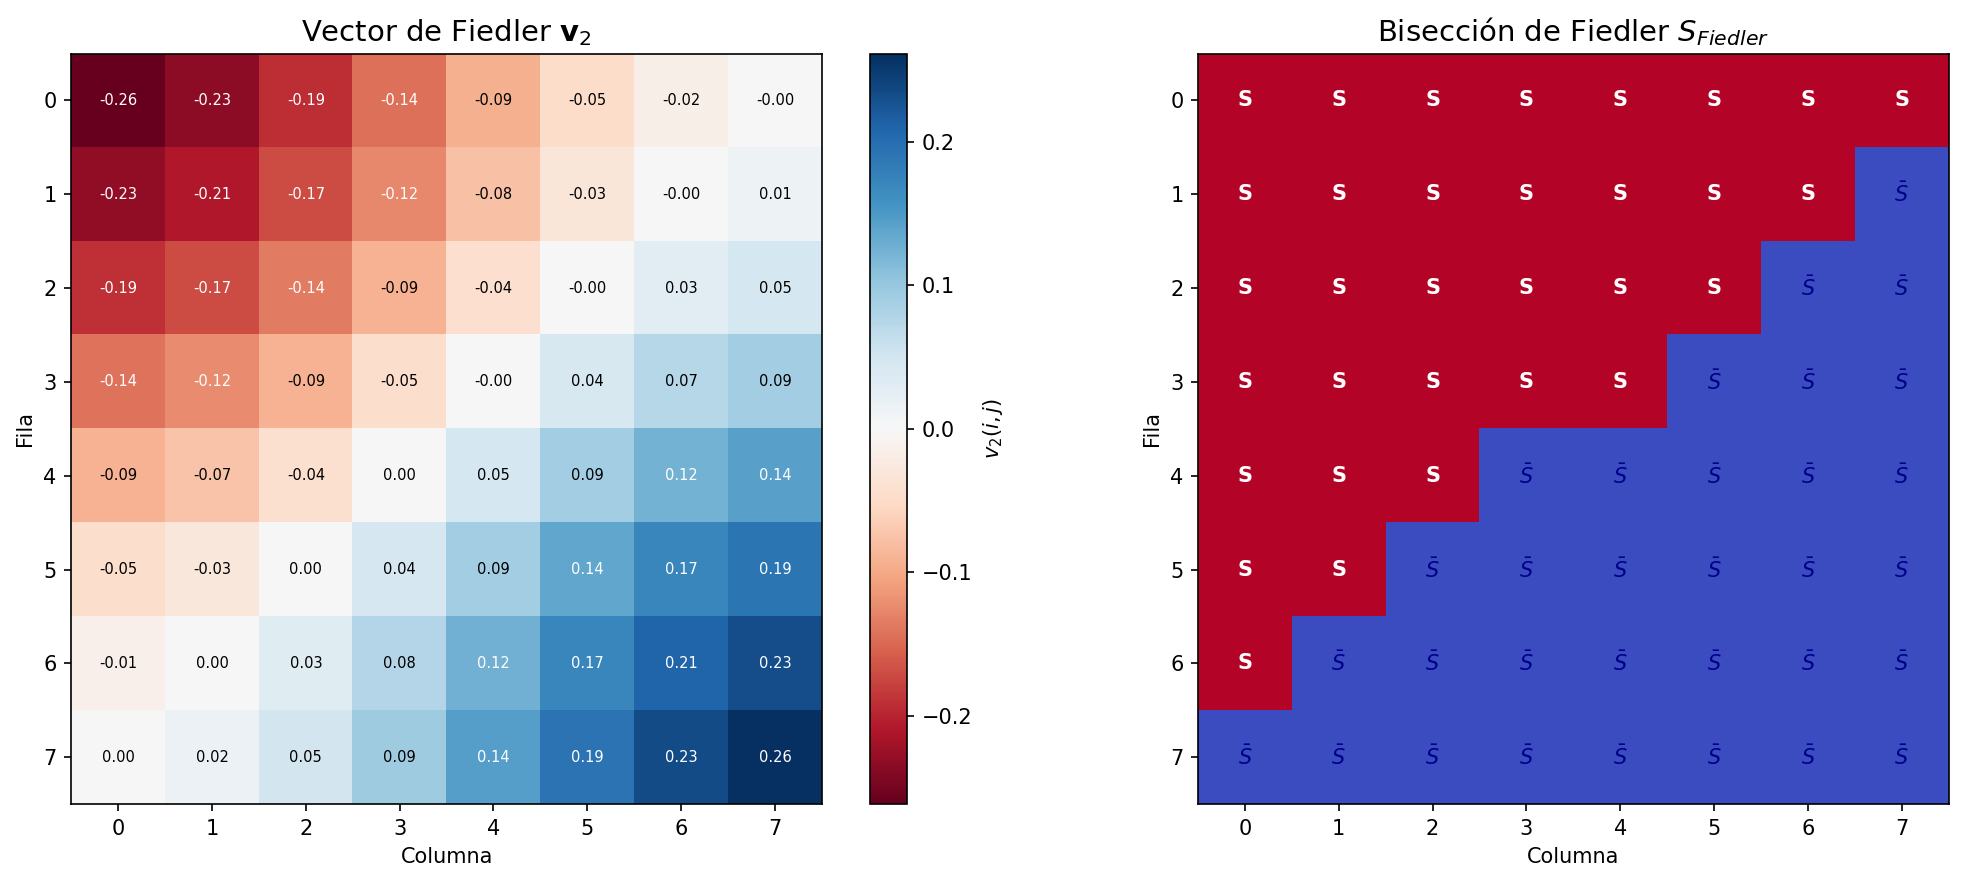
\includegraphics[width=\columnwidth]{fiedler_grid.png}
\caption{Vector de Fiedler sobre el tablero $P_8 \boxtimes P_8$. La estructura cuadrada del soporte refleja la simetría $D_4$ asociada a la degeneración $\lambda_2 = \lambda_3$.}
\label{fig:fiedler}
\end{figure}

\subsection{Comparación con particiones humanas}\label{sec:res-comparacion}

El conjunto primario, definido por las 29 díadas con partición observada en el rango $10 \le |\Sobs| \le 54$ sobre la ventana $[40,60]$, se estratifica en 21 díadas axiales (10~LR, 11~TB) y 8 díadas mixtas. Las 16 díadas excluidas pertenecen mayoritariamente a categorías \emph{ALL} (7), \emph{RS} (6) y \emph{NOTHING} (3), que la representación bipartita no captura limpiamente. Esta distribución delimita el alcance de la lente espectral: fuerte para particiones axiales, parcial para estrategias de cobertura uniforme.

La Tabla~\ref{tab:comparacion} resume las medias por grupo y los contrastes de Mann--Whitney. Las diferencias entre díadas axiales y mixtas son estadísticamente significativas en las cuatro variables consideradas: la conductancia observada (un orden de magnitud menor en el grupo axial), la eficiencia $\eta = h(\Sing)/h(\Sobs)$, la información mutua y la divergencia de Jensen--Shannon. La Figura~\ref{fig:spec-comp} ilustra estas diferencias.

\begin{table}[t]
\centering
\caption{Comparación entre díadas axiales y mixtas sobre el conjunto primario ($n = 29$). Test de Mann--Whitney bilateral.}
\label{tab:comparacion}
\begin{tabular}{@{}lcccc@{}}
\toprule
\textbf{Variable} & \textbf{Axial} ($n=21$) & \textbf{Mixed} ($n=8$) & \textbf{$U$} & \textbf{$p$-valor} \\
\midrule
$h_{\mathrm{obs}}$ & $0{,}142 \pm 0{,}108$ & $0{,}714 \pm 0{,}164$ & $3{,}0$    & $3{,}07 \times 10^{-5}$ \\
$\eta$             & $1{,}120 \pm 0{,}281$ & $0{,}196 \pm 0{,}049$ & $165{,}0$  & $3{,}07 \times 10^{-5}$ \\
$MI$               & $0{,}839 \pm 0{,}264$ & $0{,}260 \pm 0{,}176$ & $156{,}0$  & $4{,}23 \times 10^{-4}$ \\
$JSD$              & $0{,}842 \pm 0{,}261$ & $0{,}284 \pm 0{,}174$ & $157{,}0$  & $3{,}51 \times 10^{-4}$ \\
$DLIndex$          & $0{,}919 \pm 0{,}143$ & $0{,}514 \pm 0{,}129$ & $162{,}0$  & $1{,}33 \times 10^{-4}$ \\
\bottomrule
\end{tabular}
\end{table}

\begin{figure}[t]
\centering
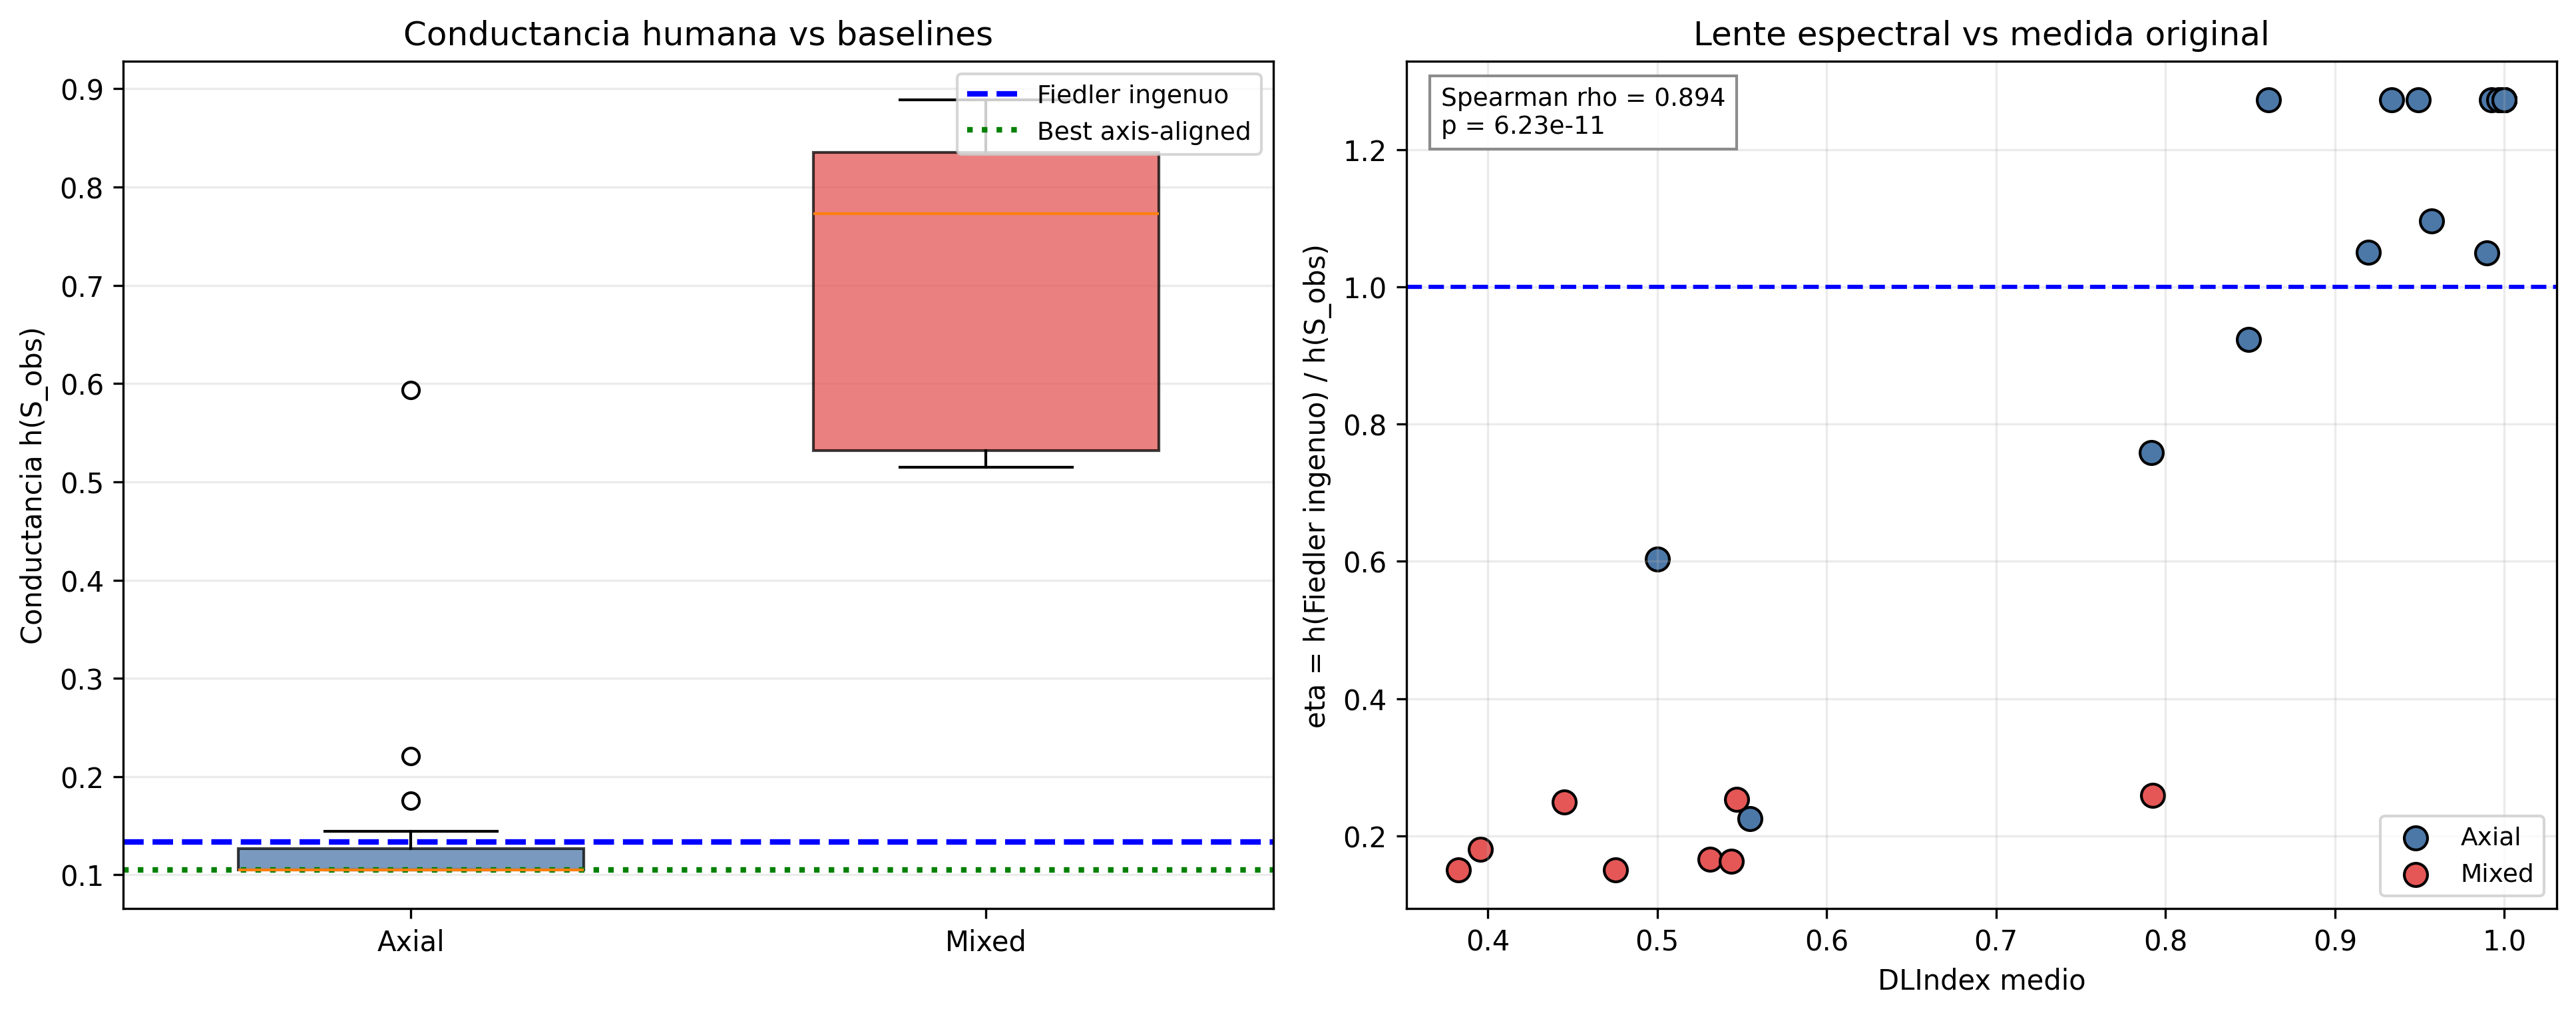
\includegraphics[width=\columnwidth]{spectral_comparison_summary.png}
\caption{Comparación de díadas axiales y mixtas sobre el conjunto primario ($n=29$). Izquierda: distribución de $h_{\mathrm{obs}}$. Derecha: relación entre $DLIndex$ y $\eta$.}
\label{fig:spec-comp}
\end{figure}

El grupo axial es heterogéneo internamente. De las 21 díadas axiales, 14 alcanzan exactamente el baseline axis-aligned $h = 22/210$, 3 mejoran el corte de Fiedler ingenuo sin alcanzarlo y 4 quedan por encima del baseline ingenuo. Esta granularidad indica que la etiqueta binaria axial--mixta resume bien la separación, pero oculta una distribución de calidades dentro del grupo axial que merece un tratamiento separado en trabajos futuros.

La eficiencia $\eta$ del grupo axial supera la unidad, lo que indica que la conductancia observada se aproxima al baseline axis-aligned $h = 22/210$ y mejora el redondeo ingenuo de Fiedler. Esta observación no debe interpretarse como evidencia de que las díadas humanas optimicen globalmente la conductancia: la geometría del tablero ya privilegia la familia de cortes axiales y la coordinación humana converge a uno de sus elementos.

Para evaluar si la lente espectral aporta una dimensión nueva frente a las métricas oficiales se computó la correlación de Spearman entre $\eta$ y $DLIndex_{\mathrm{mean}}$ sobre el conjunto primario, obteniendo $\rho = 0{,}894$ ($p = 6{,}2 \times 10^{-11}$). El resultado tiene una lectura crítica: la lente espectral separa correctamente los grupos, pero captura información altamente concordante con la métrica original; el aporte distintivo del proyecto no reside en la conductancia tardía como sustituto de $DLIndex$, sino en la formulación geométrica explícita y, sobre todo, en la señal temprana descrita más adelante.

La dinámica temporal por ronda (Figura~\ref{fig:temporal}) refuerza esta lectura: las díadas axiales reducen rápidamente la conductancia observada hasta cerca del baseline axial, mientras que las mixtas oscilan en valores altos sin estabilizarse.

\begin{figure}[t]
\centering
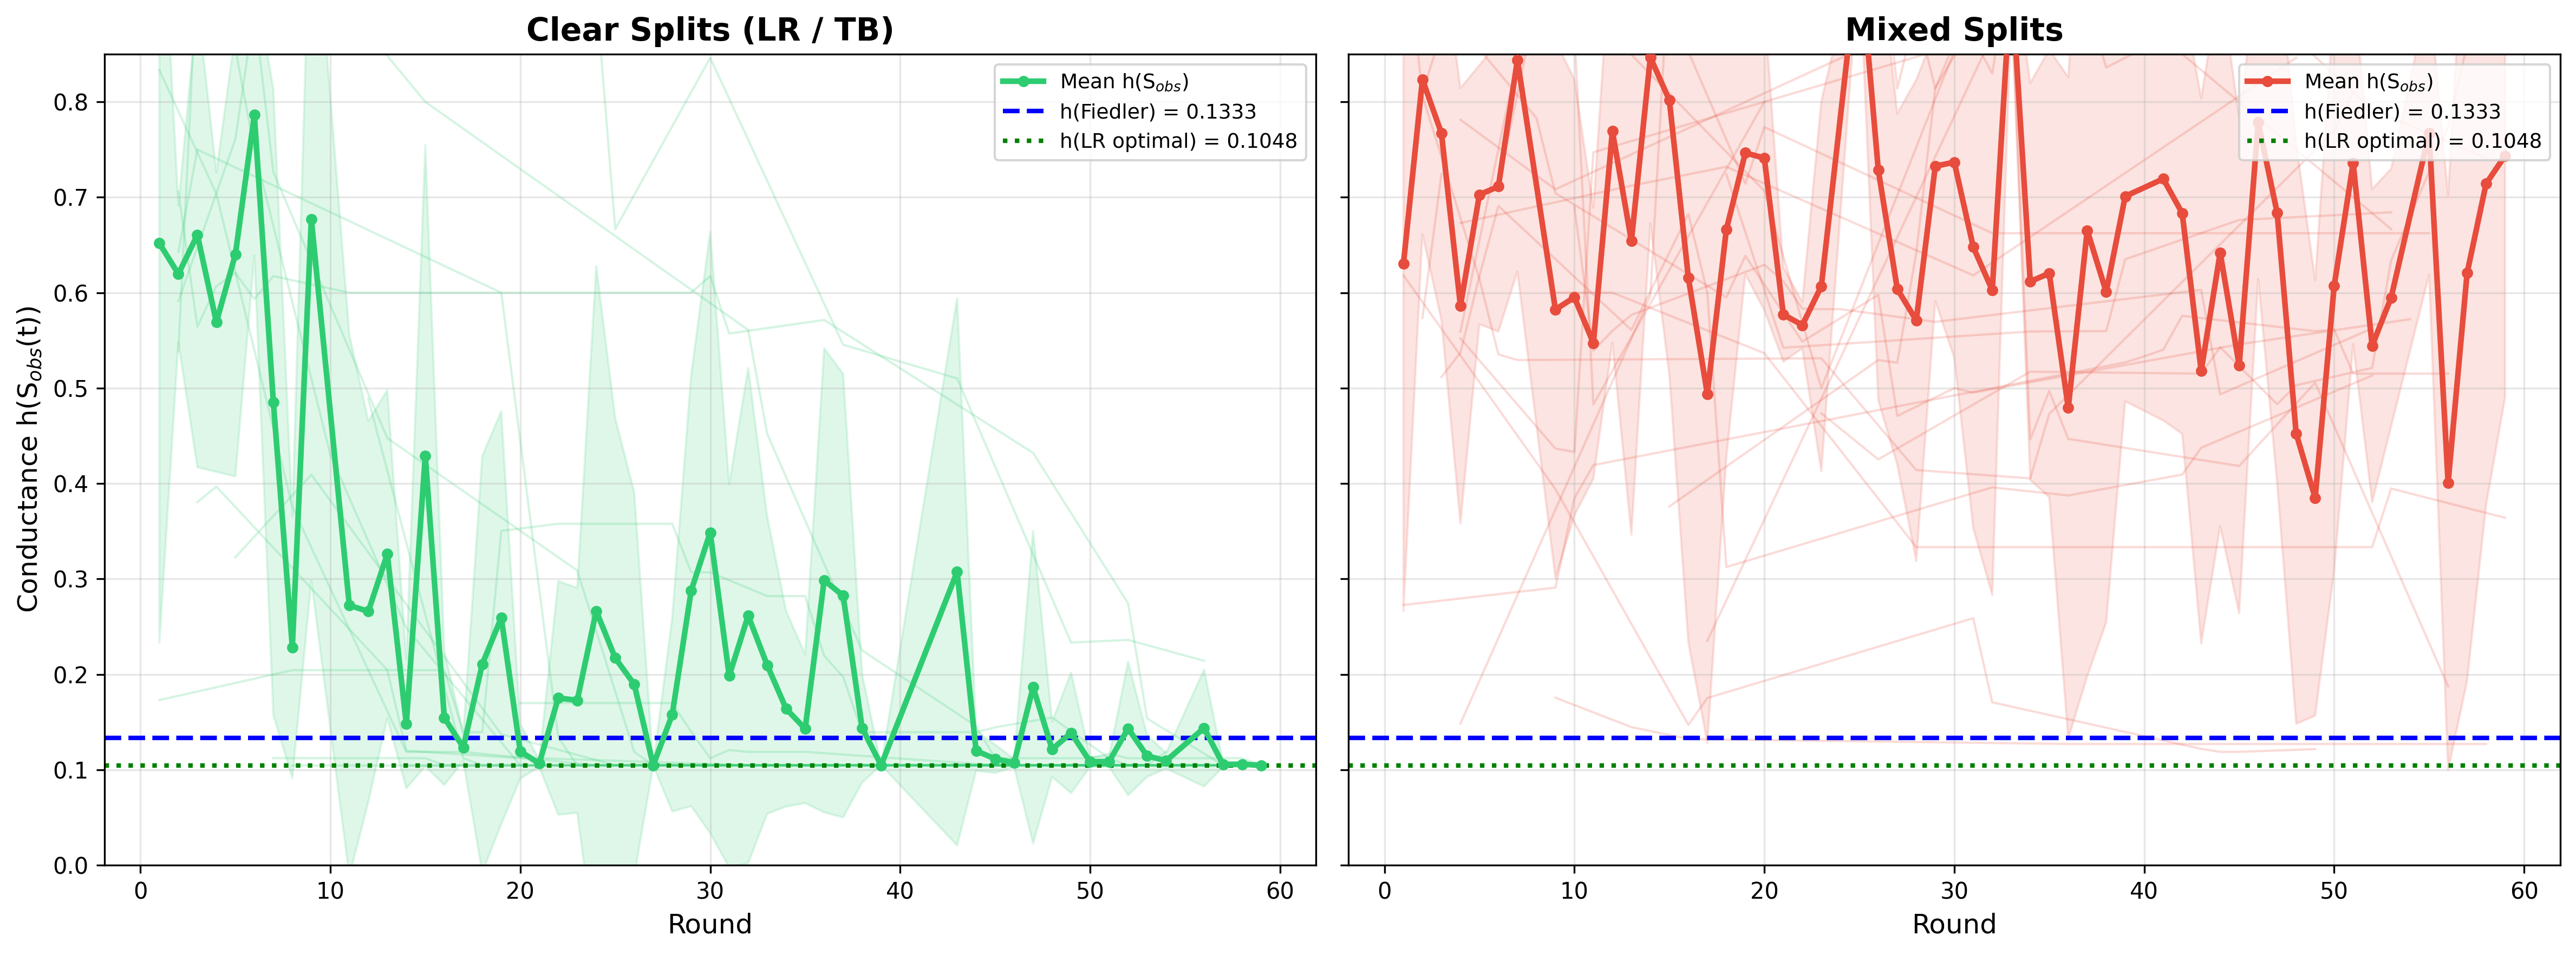
\includegraphics[width=\columnwidth]{temporal_dynamics.png}
\caption{Evolución temporal de $h_{\mathrm{obs}}(t)$ por ronda. Las díadas axiales (LR, TB) convergen rápidamente al rango del baseline axial; las mixtas no se estabilizan.}
\label{fig:temporal}
\end{figure}

\subsection{Contraejemplo rectangular: la degeneración no se observa fuera del cuadrado}\label{sec:res-counter}

Para distinguir el efecto de la simetría del tablero del comportamiento general del producto fuerte, se computó el espectro del Laplaciano del grafo rectangular $G' = P_6 \boxtimes P_8$ (48 vértices). El segundo autovalor es entonces estrictamente menor que el tercero,
\[
\lambda_2(G') = 0{,}4041,\qquad \lambda_3(G') = 0{,}7288, \qquad \lambda_3 - \lambda_2 = 0{,}3247,
\]
con multiplicidad $1$ para $\lambda_2$. La bisección de Fiedler asociada produce un corte único de $16$ aristas con conductancia $h = 16/152 \approx 0{,}1053$, sin necesidad de explorar una familia paramétrica. La Figura~\ref{fig:counter} presenta el contraste entre ambos espectros. La lectura es cautelosa: la degeneración tratada en este trabajo se observa en el caso cuadrado analizado y no aparece en la geometría rectangular probada, lo que es coherente con un origen estructural en la simetría $D_4$ y argumenta en contra de un artefacto numérico. Por consiguiente, la solución espectral propuesta es necesaria precisamente sobre $P_8 \boxtimes P_8$ y no se trasladaría sin cambios a tableros con simetría reducida.

\begin{figure}[t]
\centering
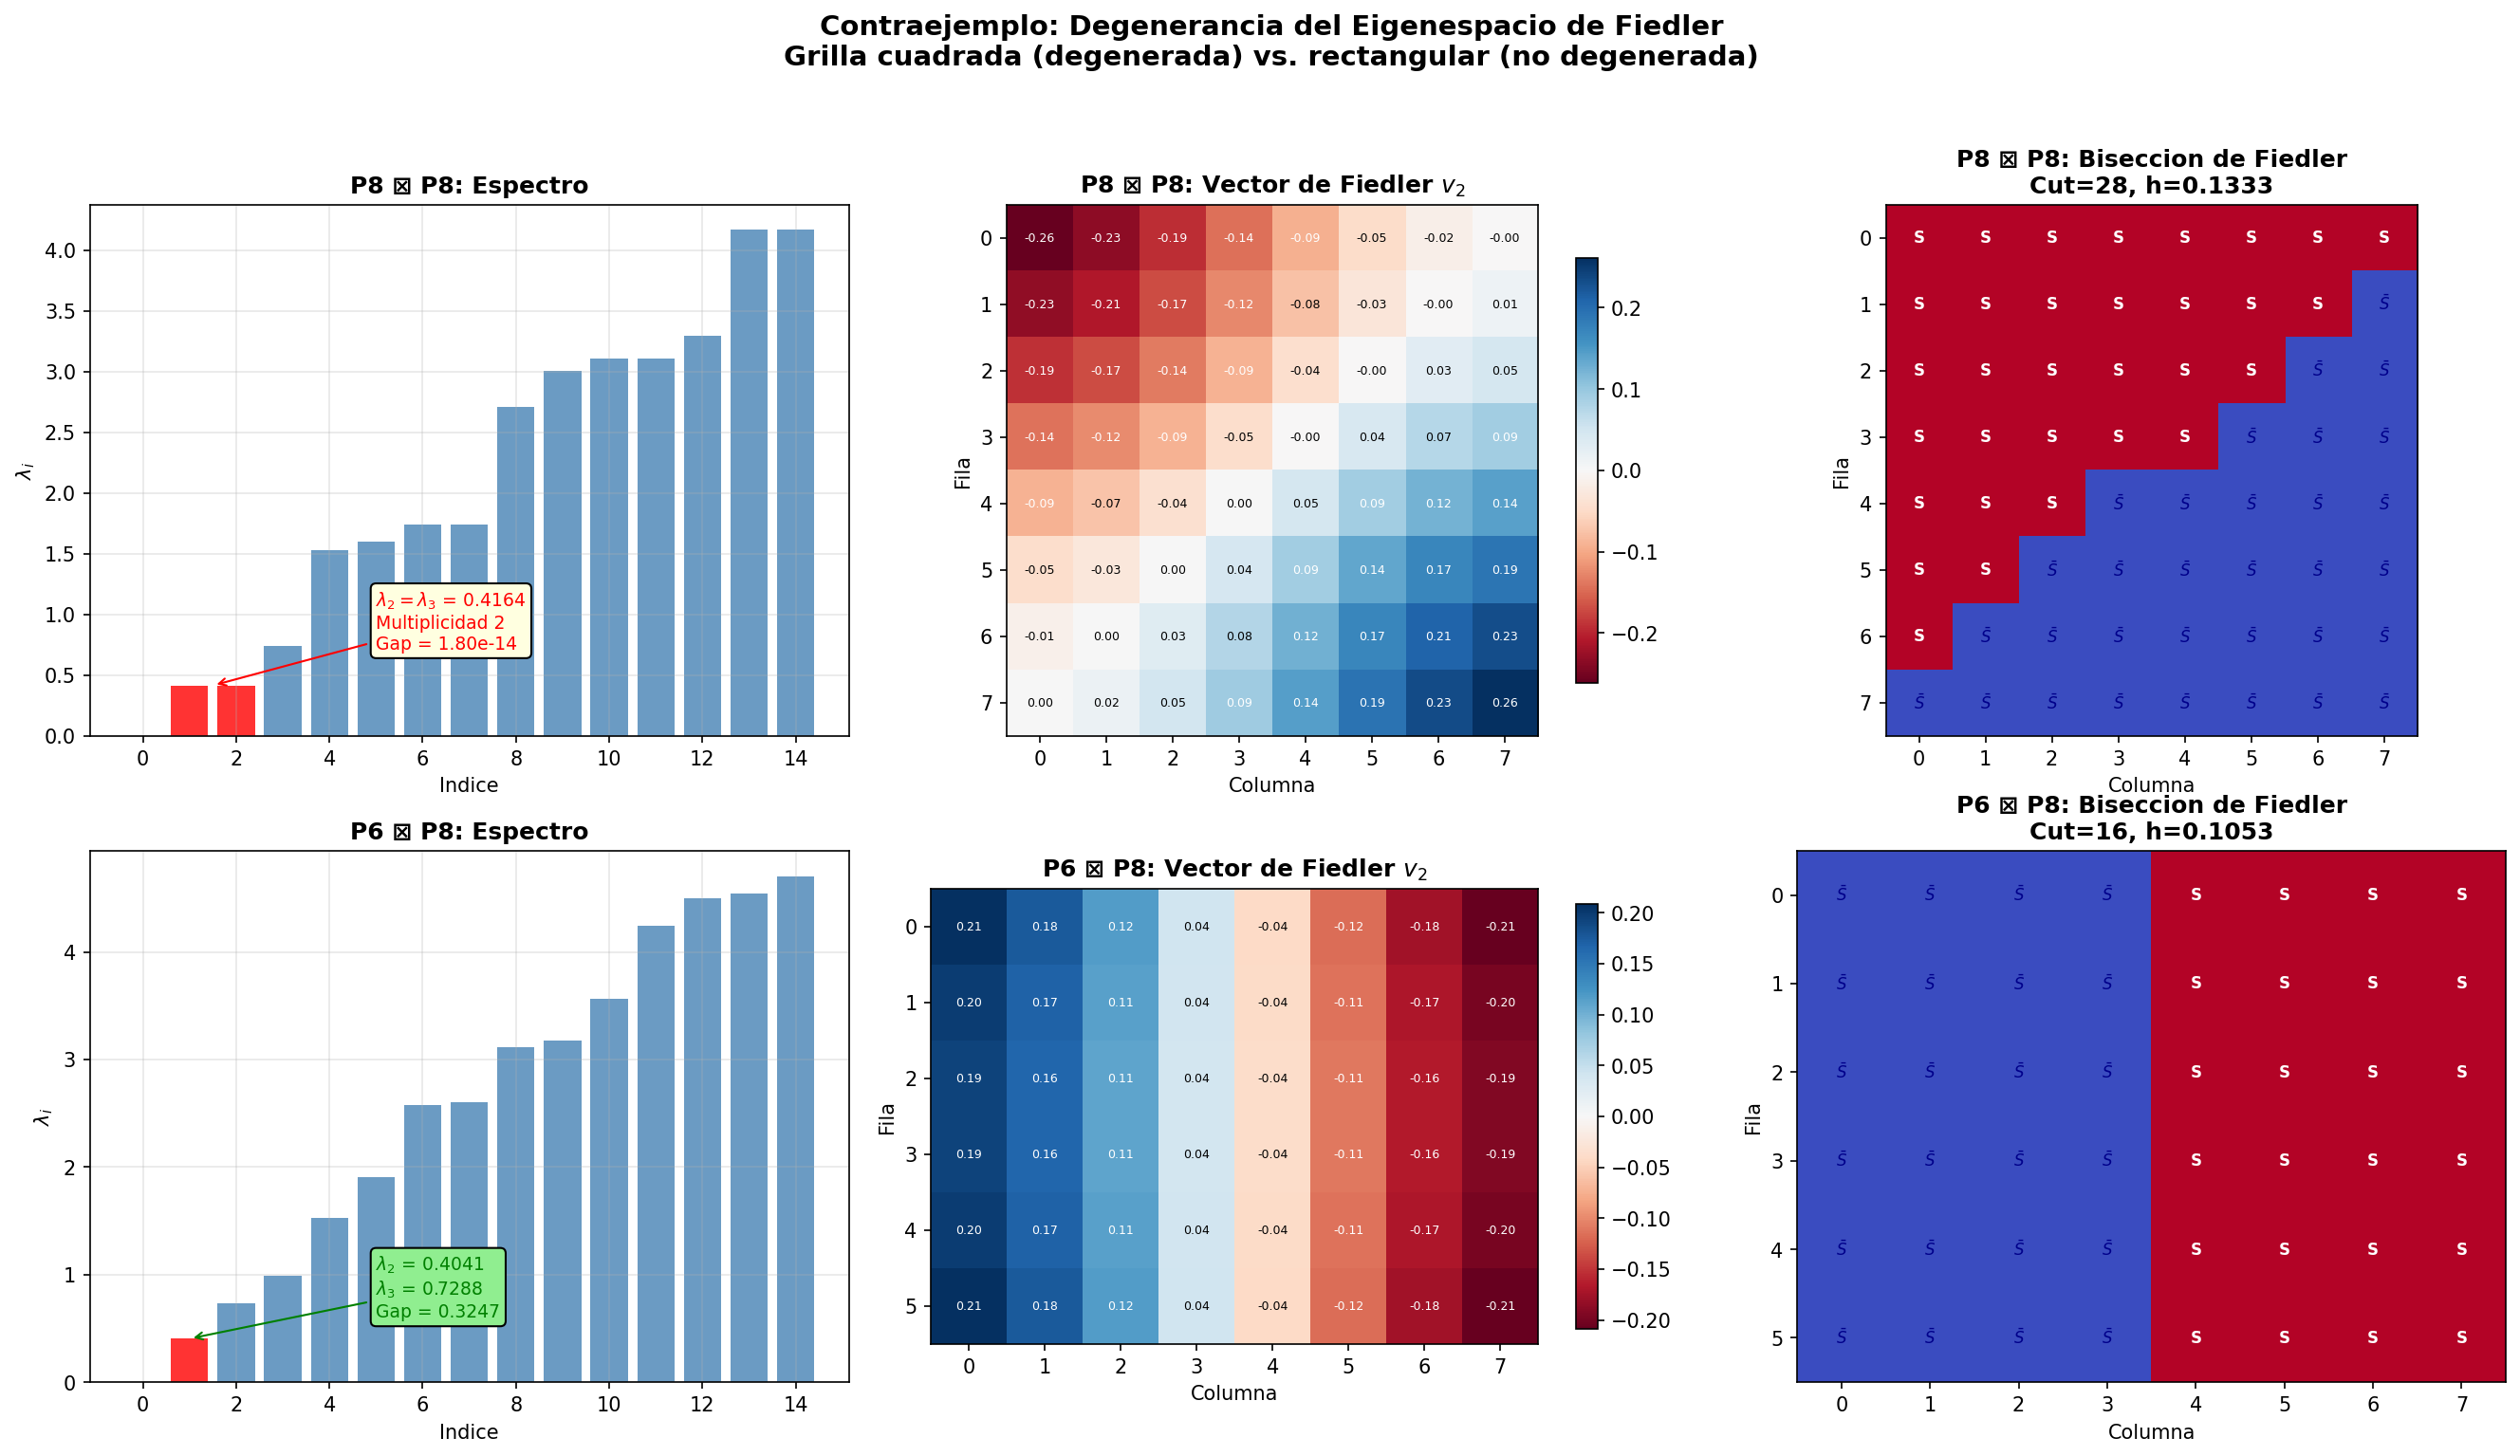
\includegraphics[width=\columnwidth]{counterexample_P6xP8.png}
\caption{Contraejemplo rectangular. Sobre $P_6 \boxtimes P_8$ el segundo autovalor es simple y el redondeo de Fiedler ingenuo es válido; la degeneración $\lambda_2 = \lambda_3$ no aparece en esta geometría rectangular.}
\label{fig:counter}
\end{figure}

\subsection{Robustez de la partición observada}\label{sec:res-robustez}

La estabilidad de la partición $\Sobs^{(d,W)}$ a lo largo de las ventanas tardías $W_1, W_2, W_3$ se evaluó mediante el índice de Jaccard pareado y la coincidencia entre orientaciones inferidas. Sobre el conjunto de díadas con tres ventanas válidas, la mediana del índice de Jaccard alcanza $1{,}000$ para LR ($\bar J = 0{,}960$, $\sigma = 0{,}086$, $n=10$) y para TB ($\bar J = 0{,}908$, $\sigma = 0{,}202$, $n=10$), frente a $\bar J = 0{,}651$ ($\sigma = 0{,}213$, $n=8$) en las díadas mixtas (Figura~\ref{fig:robustez}). El ordenamiento se cumple también sobre la ventana intermedia: las díadas con orientación axial estable preservan casi exactamente el mismo conjunto $\Sobs$ entre las tres ventanas, mientras que las mixtas reorganizan aproximadamente la mitad de sus celdas dominantes al desplazar la ventana. La etiqueta $y_d$ tiene, por tanto, una base empírica robusta y no depende de la elección particular de un horizonte temporal.

\begin{figure}[t]
\centering
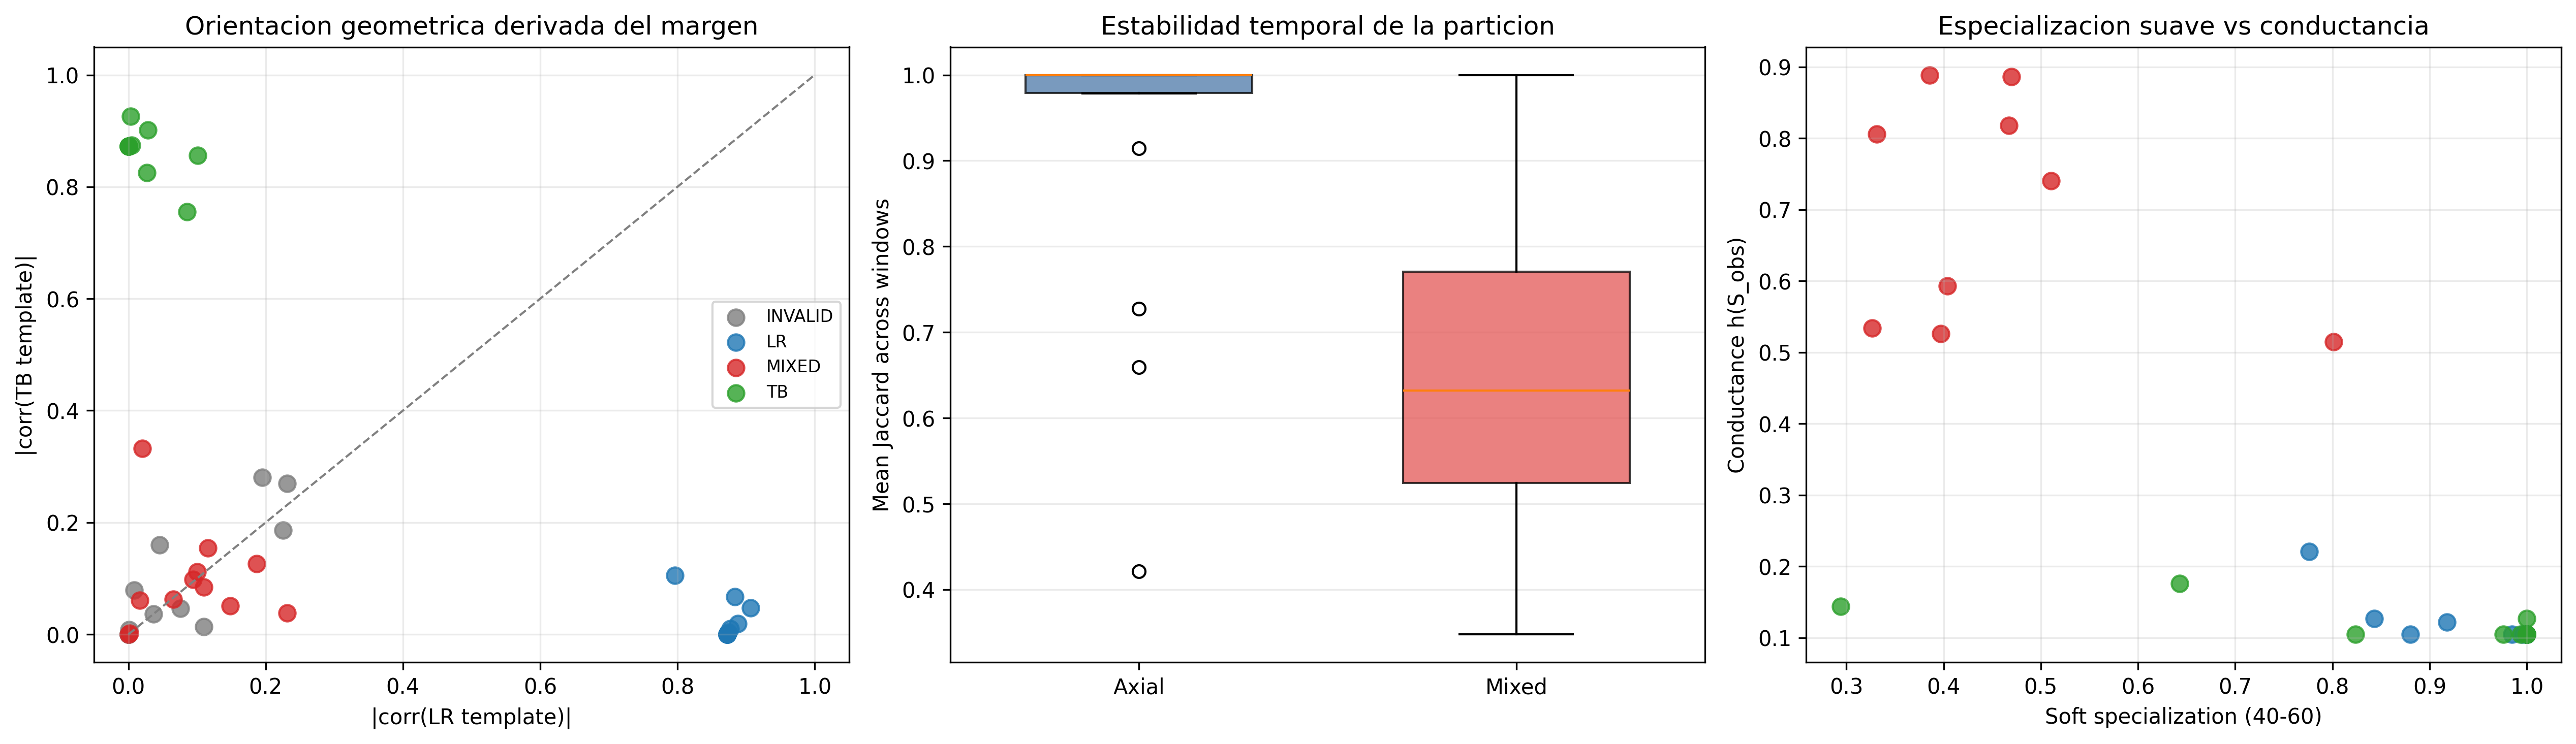
\includegraphics[width=\columnwidth]{partition_robustness_summary.png}
\caption{Estabilidad por ventana de la partición $\Sobs$. Las díadas axiales estables preservan el mismo conjunto dominante a lo largo de $W_1, W_2, W_3$; las mixtas no.}
\label{fig:robustez}
\end{figure}

\subsection{Predicción temprana de la especialización axial}\label{sec:res-prediccion}

La Tabla~\ref{tab:auc} resume las áreas bajo la curva ROC de los tres modelos de clasificación logística sobre el conjunto completo de 45 díadas (20 positivas, 25 negativas) y, como contraste, sobre el subconjunto de 32 díadas con etiqueta de orientación tardía válida (20 positivas, 12 negativas). Sobre las 45 díadas, el modelo basado únicamente en la señal geométrica temprana $g_d$ alcanza $\mathrm{AUC}_{\mathrm{LOOCV}} = 0{,}804$ y supera al trío de métricas oficiales tempranas ($0{,}736$); la combinación de ambas familias de características eleva el desempeño a $0{,}860$, con un incremento de $5{,}6$ puntos porcentuales sobre la geometría aislada y de $12{,}4$ puntos sobre las métricas oficiales. La Figura~\ref{fig:early} ilustra estas comparaciones.

\begin{table}[t]
\centering
\caption{Predicción temprana de la orientación axial estable. Modelos logísticos bajo \emph{leave-one-out}, evaluados sobre el conjunto completo (45 díadas) y el subconjunto de etiquetas válidas (32 díadas).}
\label{tab:auc}
\begin{tabular}{@{}llcc@{}}
\toprule
\textbf{Conjunto} & \textbf{Variables} & \textbf{AUC$_{\mathrm{in}}$} & \textbf{AUC$_{\mathrm{LOOCV}}$} \\
\midrule
Todas (45)        & $g_d$                                 & $0{,}834$ & $0{,}804$ \\
Todas (45)        & Trío oficial                          & $0{,}808$ & $0{,}736$ \\
Todas (45)        & $g_d$ + trío oficial                  & $0{,}890$ & $\mathbf{0{,}860}$ \\
\addlinespace
Válidas (32)      & $g_d$                                 & $0{,}825$ & $0{,}779$ \\
Válidas (32)      & Trío oficial                          & $0{,}858$ & $0{,}775$ \\
Válidas (32)      & $g_d$ + trío oficial                  & $0{,}908$ & $0{,}813$ \\
\bottomrule
\end{tabular}
\end{table}

\begin{figure}[t]
\centering
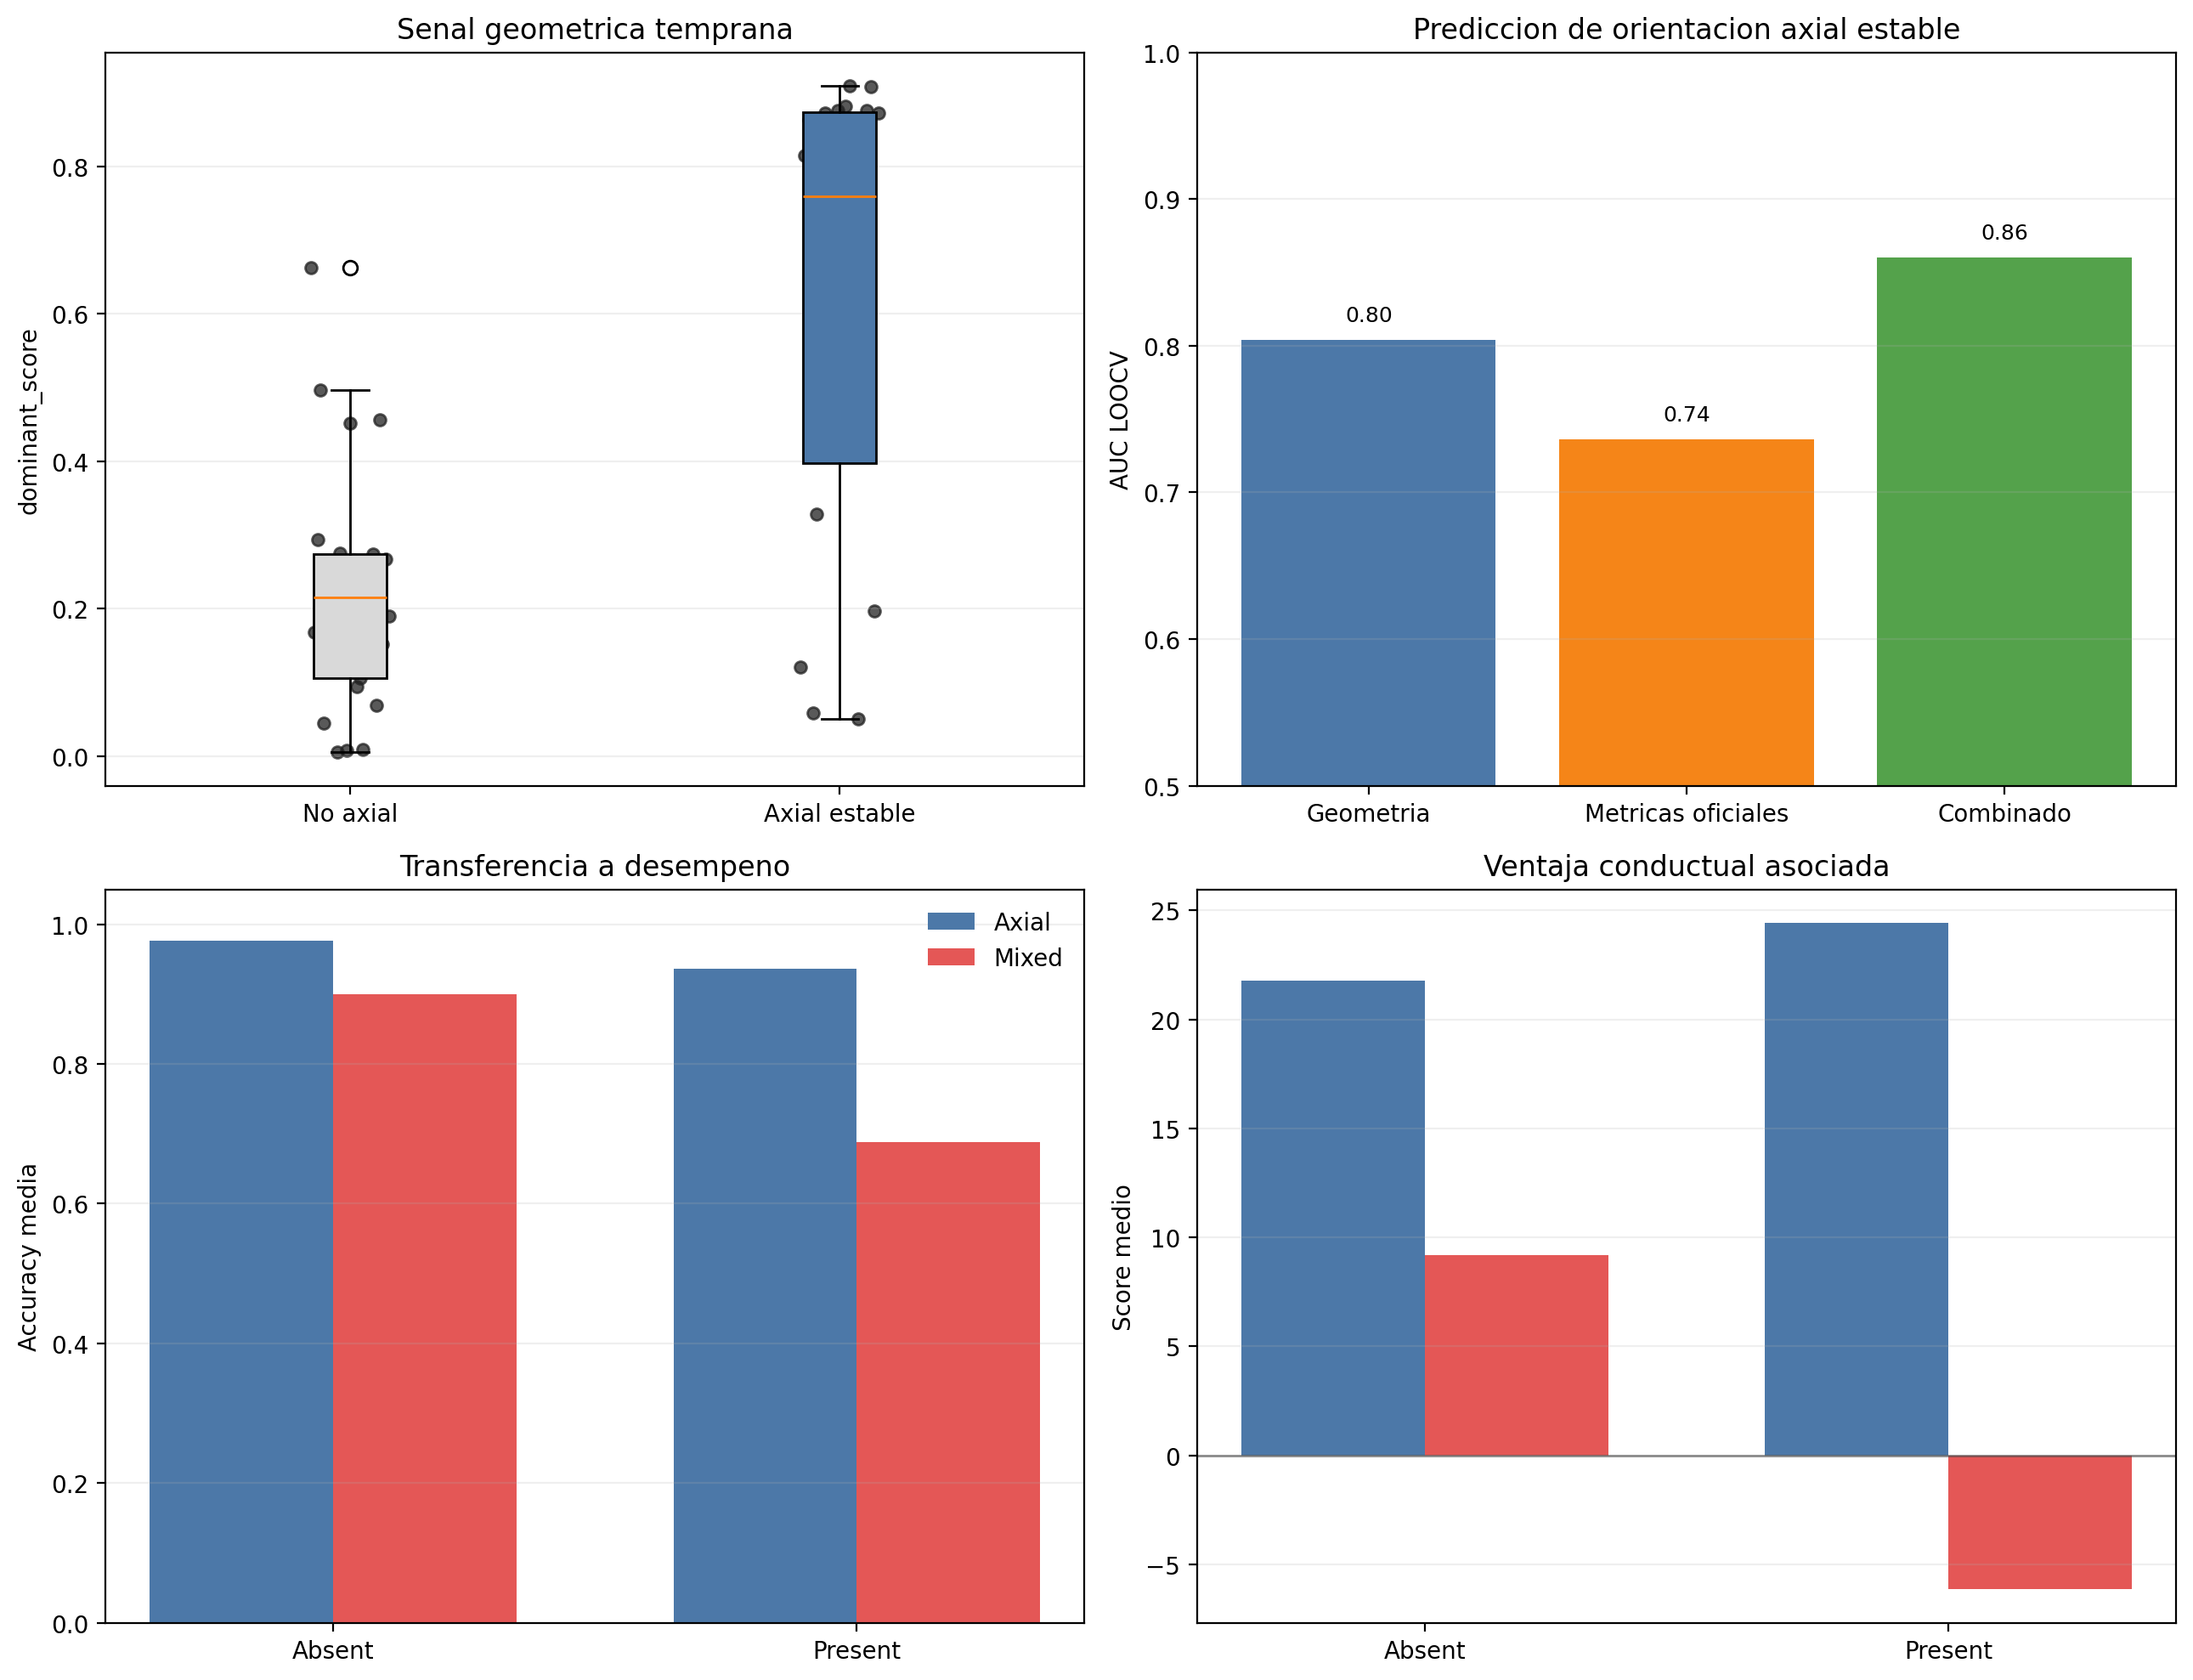
\includegraphics[width=\columnwidth]{early_prediction_summary.png}
\caption{Predicción temprana de la especialización axial estable. La señal geométrica $g_d$ aporta valor predictivo complementario a las métricas oficiales.}
\label{fig:early}
\end{figure}

La lectura es matizada. Sobre el conjunto completo, la señal geométrica temprana, basada únicamente en cinco rondas y en una operación de proyección sobre dos plantillas axiales, supera a las métricas oficiales tempranas. Cuando el análisis se restringe a las 32 díadas con etiqueta tardía más confiable, la ventaja de la geometría sobre el trío oficial se atenúa ($0{,}779$ frente a $0{,}775$) y la combinación se mantiene como mejor modelo ($0{,}813$). Esta atenuación es informativa: indica que el aporte central de $g_d$ se concentra en la fase temprana de predicción y, en particular, en las díadas para las que la categorización tardía es ambigua, no en una superioridad uniforme sobre las métricas existentes.

\subsection{Asociación con el desempeño conductual posterior}\label{sec:res-transferencia}

Para evaluar el alcance conductual de la orientación inferida, se cruzaron las etiquetas estables AXIAL/MIXED con la tabla completa \emph{performances.csv} (5\,400 rondas). La Tabla~\ref{tab:transfer} resume tres medidas oficiales ---precisión, score y conjunción de aciertos--- estratificadas por la presencia o ausencia del unicornio. Las díadas axialmente estables se asocian con valores más altos de precisión y de score que las mixtas en ambos regímenes; la diferencia es particularmente marcada en rondas con unicornio presente, donde la precisión asciende de $0{,}688$ a $0{,}936$ y el score promedio pasa de $-6{,}14$ a $24{,}43$. Esta asociación es coherente con el marco teórico ---la ruptura de simetría hacia un eje compatible con $D_4$ acompaña una organización estable que también acompaña al desempeño en condiciones distintas a las usadas para inferirla--- pero se reporta de forma descriptiva: la unidad experimental es la díada y no cada ronda individual, y por tanto el resultado no debe leerse como inferencia causal.

\begin{table}[t]
\centering
\caption{Asociación entre orientación inferida y desempeño conductual. Medias por grupo en la tabla \emph{performances.csv} (5\,400 rondas). Lectura descriptiva.}
\label{tab:transfer}
\begin{tabular}{@{}llrrr@{}}
\toprule
\textbf{Régimen} & \textbf{Grupo} & \textbf{Accuracy} & \textbf{Score} & \textbf{Joint} \\
\midrule
Unicornio ausente  & AXIAL  & $0{,}977$ & $21{,}79$ & $\phantom{-}8{,}17$ \\
                   & MIXED  & $0{,}900$ & $\phantom{-}9{,}19$  & $13{,}18$ \\
\addlinespace
Unicornio presente & AXIAL  & $0{,}936$ & $24{,}43$ & $\phantom{-}2{,}19$ \\
                   & MIXED  & $0{,}688$ & $-6{,}14$ & $\phantom{-}5{,}39$ \\
\bottomrule
\end{tabular}
\end{table}

Como diagnóstico complementario se evaluó el valor incremental de la conductancia tardía $h_{\mathrm{obs}}$ y de su recíproco normalizado $\eta$ frente al modelo oficial bajo \emph{leave-one-out}. Para la predicción del score promedio en rondas con unicornio presente, el modelo oficial alcanza $R^2_{\mathrm{LOOCV}} = 0{,}654$; añadir $h_{\mathrm{obs}}$ reduce el desempeño a $0{,}497$ y añadir $\eta$ a $0{,}575$. Resultados análogos se observan para precisión y conjunción. La interpretación es directa: el aporte distintivo del proyecto no reside en una conductancia tardía que reemplace a las métricas oficiales, sino en la formulación espectral coherente, en la señal temprana $g_d$ y en la asociación consistente entre orientación inferida y desempeño conductual.

\section{Conclusiones}\label{sec:conclusiones}

El trabajo cumple los siete objetivos específicos formulados en la Sección~\ref{sec:objetivos}. El tablero experimental se modeló como el producto fuerte $P_8 \boxtimes P_8$ y se caracterizó su espectro, documentando con precisión de máquina la degeneración $\lambda_2 = \lambda_3 \approx 0{,}4164$ asociada a la simetría $D_4$. Sobre esa base se distinguieron tres familias de referencias espectrales ---el redondeo ingenuo, los cortes axiales LR y TB, y la familia paramétrica $\{S_\theta\}$--- y se mostró numéricamente que las dos últimas alcanzan la conductancia mínima dentro del eigenespacio de Fiedler. La partición observada de cada díada se definió por dominancia de frecuencias en una ventana ausente y se evaluó mediante conductancia, información mutua y divergencia de Jensen--Shannon. La etiqueta de orientación axial estable se construyó a partir de tres ventanas tardías y se verificó robusta bajo el índice de Jaccard. La señal geométrica temprana $g_d$ se diseñó como una proyección sobre dos plantillas axiales y se comparó con las métricas oficiales bajo LOOCV. Finalmente, el pipeline computacional se consolidó como herramienta reproducible y la orientación inferida se cruzó con la tabla completa \emph{performances.csv} para una lectura descriptiva de su asociación con desempeño.

Los resultados son consistentes entre sí. Las díadas axialmente estables alcanzan conductancias compatibles con el baseline axis-aligned ($h_{\mathrm{obs}} \approx 0{,}142$, $\eta \approx 1{,}12$), mientras que las mixtas se mantienen lejos del óptimo del eigenespacio degenerado ($h_{\mathrm{obs}} \approx 0{,}71$, $\eta \approx 0{,}20$). La diferencia es estadísticamente significativa en todas las variables consideradas. La señal geométrica temprana, calculada sobre cinco rondas, alcanza $\mathrm{AUC}_{\mathrm{LOOCV}} = 0{,}804$ y, combinada con las métricas oficiales, $0{,}860$ sobre el conjunto completo de 45 díadas. El contraejemplo sobre $P_6 \boxtimes P_8$ es consistente con la lectura de que la degeneración tratada se asocia con la simetría $D_4$ del cuadrado y no aparece en la geometría rectangular probada. La orientación inferida se asocia con un mejor desempeño conductual posterior, particularmente marcado en rondas con unicornio presente.

El alcance del trabajo está delimitado de manera explícita. Primero, la representación bipartita captura limpiamente las estrategias axiales del experimento, pero no las categorías \emph{ALL}, \emph{NOTHING} y \emph{RS}, que constituyen una fracción no despreciable de las díadas excluidas. Segundo, la conductancia tardía $h_{\mathrm{obs}}$ presenta una correlación de Spearman $\rho = 0{,}894$ con $DLIndex_{\mathrm{mean}}$ y no aporta valor predictivo incremental sobre las métricas oficiales para predecir desempeño; el aporte del proyecto reside, por tanto, en la formulación geométrica y en la señal temprana, no en una sustitución de las medidas existentes. Tercero, la muestra es pequeña ($n=29$ en el conjunto primario, $n=45$ en la auditoría) y los resultados deben interpretarse como evidencia de plausibilidad de la lente espectral, no como inferencia causal; la asociación con desempeño se reporta de forma descriptiva, con la díada ---no la ronda--- como unidad experimental.

Estas limitaciones sugieren tres líneas de trabajo futuro. La primera es teórica: explorar familias de plantillas más amplias que las dos direcciones axiales canónicas, derivadas explícitamente de las representaciones irreducibles de $D_4$ sobre el eigenespacio de Fiedler, para evaluar si existen orientaciones humanas no axiales sistemáticas que la presente formulación no captura. La segunda es metodológica: extender el análisis temporal a las 60 rondas completas, integrando rondas con unicornio presente bajo un esquema de censura adecuado, lo que permitiría modelar la cristalización de roles como un proceso dinámico y no únicamente como una clasificación binaria. La tercera, y a mi juicio la más prometedora, es experimental: el diseño actual permite formular una predicción falsable a partir de la teoría desarrollada. Si la degeneración del eigenespacio de Fiedler es la fuente estructural de la ambigüedad de roles axiales en el tablero cuadrado, modificar la simetría del entorno ---por ejemplo, mediante tableros rectangulares o cuadrados con obstáculos que rompan $D_4$--- debería reducir la fracción de díadas mixtas y desplazar a los participantes hacia una única orientación dominante, ya predicha por la bisección de Fiedler ahora simple. Una validación empírica de este desplazamiento convertiría el reanálisis ofrecido en este trabajo en una agenda experimental concreta sobre cómo la estructura espectral del entorno modela la coordinación multiagente.

En conjunto, el proyecto muestra que la teoría espectral de grafos provee un marco coherente y operativo para reanalizar el paradigma \emph{Seeking the Unicorn}, no como un competidor de las métricas conductuales del estudio original sino como una capa explicativa que vincula la simetría del entorno con la dinámica de coordinación humana y permite anticipar, desde la fase inicial del experimento, qué díadas terminarán especializándose a lo largo de uno de los ejes privilegiados por el tablero.

\bibliographystyle{IEEEtran}
\begin{thebibliography}{10}

\bibitem{andrade2021}
E. Andrade-Lotero and R. L. Goldstone, ``Self-organized division of cognitive labor,'' \textit{PLOS ONE}, vol. 16, no. 7, p. e0254532, Jul. 2021.

\bibitem{mesbahi2010}
M. Mesbahi and M. Egerstedt, \textit{Graph Theoretic Methods in Multiagent Networks}. Princeton, NJ: Princeton University Press, 2010.

\bibitem{goldstone2024}
R. L. Goldstone, E. Andrade-Lotero, R. D. Hawkins, and M. E. Roberts, ``The emergence of specialized roles within groups,'' \textit{Topics in Cognitive Science}, 2024.

\bibitem{hammack2011}
R. Hammack, W. Imrich, and S. Klav\v{z}ar, \textit{Handbook of Product Graphs}, 2nd ed. Boca Raton, FL: CRC Press, 2011.

\bibitem{fiedler1973}
M. Fiedler, ``Algebraic connectivity of graphs,'' \textit{Czechoslovak Mathematical Journal}, vol. 23, no. 2, pp. 298--305, 1973.

\bibitem{mohar1991}
B. Mohar, ``The Laplacian spectrum of graphs,'' in \textit{Graph Theory, Combinatorics, and Applications}, vol. 2, Y. Alavi et al., Eds. New York: Wiley, 1991, pp. 871--898.

\bibitem{chung1997}
F. R. K. Chung, \textit{Spectral Graph Theory}. Providence, RI: American Mathematical Society, 1997.

\bibitem{vonluxburg2007}
U. von Luxburg, ``A tutorial on spectral clustering,'' \textit{Statistics and Computing}, vol. 17, no. 4, pp. 395--416, Dec. 2007.

\bibitem{cheeger1970}
J. Cheeger, ``A lower bound for the smallest eigenvalue of the Laplacian,'' in \textit{Problems in Analysis}. Princeton, NJ: Princeton University Press, 1970, pp. 195--199.

\bibitem{cover2006}
T. M. Cover and J. A. Thomas, \textit{Elements of Information Theory}, 2nd ed. Hoboken, NJ: Wiley-Interscience, 2006.

\bibitem{lin1991}
J. Lin, ``Divergence measures based on the Shannon entropy,'' \textit{IEEE Transactions on Information Theory}, vol. 37, no. 1, pp. 145--151, Jan. 1991.

\bibitem{pedregosa2011}
F. Pedregosa \emph{et al.}, ``Scikit-learn: Machine learning in Python,'' \textit{Journal of Machine Learning Research}, vol. 12, pp. 2825--2830, 2011.

\bibitem{harris2020}
C. R. Harris \emph{et al.}, ``Array programming with NumPy,'' \textit{Nature}, vol. 585, no. 7825, pp. 357--362, Sep. 2020.

\bibitem{virtanen2020}
P. Virtanen \emph{et al.}, ``SciPy 1.0: fundamental algorithms for scientific computing in Python,'' \textit{Nature Methods}, vol. 17, no. 3, pp. 261--272, Mar. 2020.

\end{thebibliography}

\end{document}
